\documentclass[8pt]{beamer}

\usetheme{metropolis}

\usepackage{amssymb}
\usepackage{fontawesome}
\usepackage{pgfplots}
\usepackage{pgfplotstable}
\usepackage[normalem]{ulem}
\usepackage{varwidth}
\usepackage{xcolor}

\usetikzlibrary{arrows}
\usetikzlibrary{arrows.meta}
\usetikzlibrary{calc}

\date{19.01.23}
\title{Kunstig intelligens og maskinlæring}
\author{Esten H. Leonardsen}

\titlegraphic{
	\centering
	\vspace{7.5cm}
	\includegraphics[height=1cm]{data/bio.png}
	\hfill
	\includegraphics[height=1cm]{data/uio.png}
}

\def\nodesize{14pt}
\colorlet{nodefill}{green!20}

\begin{document}
	\begin{frame}
	 	\maketitle
	\end{frame}

	\begin{frame}{Introduksjon} % Math
		\centering
		\vfill
		\begin{itemize}
			\item $\theta_{t+1} = \theta_t - \alpha \nabla_\theta \mathcal{L}(\theta_t)$
			\item $\delta_i = \frac{\partial \mathcal{L}}{\partial z_i}$, $\delta_j = \sum_i w_{ij} \delta_i$, $\frac{\partial \mathcal{L}}{\partial w_{ij}} = \delta_i a_j$
			\item $p_i = \frac{e^{z_i}}{\sum_{j=1}^K e^{z_j}}$
			\item $\mathcal{L}(\theta) = -\frac{1}{N} \sum_{i=1}^N \sum_{k=1}^K y_{ik} \log p_{ik}$
			\item $y_{i,j,k} = \sum_{l=1}^C \sum_{p=1}^H \sum_{q=1}^W x_{i+p-1,j+q-1,l} w_{p,q,l,k}$
			\item $\hat{x} = \frac{x - \mu}{\sqrt{\sigma^2 + \epsilon}}$, $y = \gamma \hat{x} + \beta$
			\item $r_i \sim \text{Bernoulli}(p)$, $h_i = r_i \odot f(x_i)$, $f_{\text{out}}(x) = \frac{1}{1-p} \sum_{i=1}^n h_i$
			\item $L(x, g(f(x))) = \|x - g(f(x))\|^2$
		\end{itemize}
		\vfill
	\end{frame}

	\begin{frame}{Terminologi: Taksonomi} % Taxonomy, Artificial intelligence
		\centering
		\vfill
		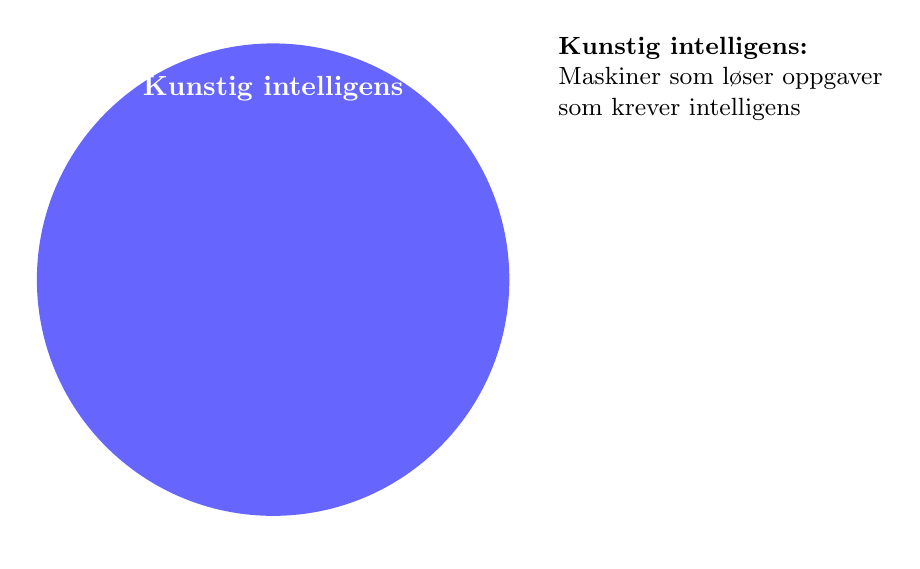
\begin{tikzpicture}
			\node[circle, fill=blue!60, minimum size=6cm] (ai) at (0, 0) {};
			\node[text=white, anchor=north] at ($ (ai.north) - (0, 0.3) $) {\textbf{Kunstig intelligens}};
			\node[anchor=north west, align=left, font=\small] (ai-text) at ($ (ai.north) + (3.5, 0.2) $) {\textbf{Kunstig intelligens:}\\Maskiner som løser oppgaver\\som krever intelligens};
			\node[] at (-3, 3) {};
			\node[] at (7.7, -3.2) {};
		\end{tikzpicture}
		\vfill
	\end{frame}

	\begin{frame}{Terminologi: Taksonomi} % Taxonomy, Machine learning
		\centering
		\vfill
		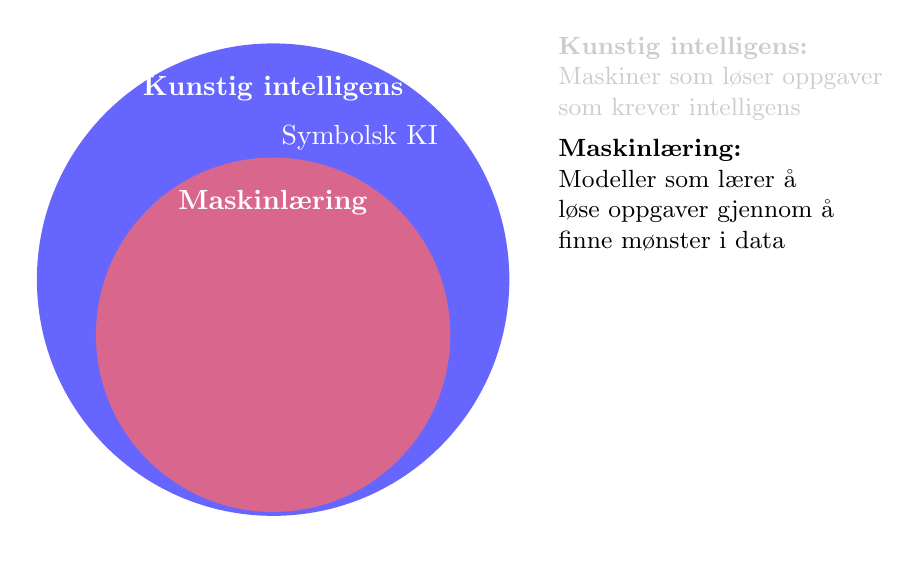
\begin{tikzpicture}
			\node[circle, fill=blue!60, minimum size=6cm] (ai) at (0, 0) {};
			\node[text=white, anchor=north] at ($ (ai.north) - (0, 0.3) $) {\textbf{Kunstig intelligens}};
			\node[text=white] at ($ (ai.north) - (-1.1, 1.2) $) {Symbolsk KI};
			\node[circle, fill=purple!60, minimum size=4.5cm, anchor=south] (ml) at ($ (ai.south) + (0, 0.05) $) {};
			\node[text=white, anchor=north] at ($ (ml.north) - (0, 0.3) $) {\textbf{Maskinlæring}};
			\node[anchor=north west, align=left, font=\small, text=gray!40] (ai-text) at ($ (ai.north) + (3.5, 0.2) $) {\textbf{Kunstig intelligens:}\\Maskiner som løser oppgaver\\som krever intelligens};
			\node[anchor=north west, align=left, font=\small] (ml-text) at ($ (ai-text.south west) - (0, 0) $) {\textbf{Maskinlæring:}\\Modeller som lærer å\\løse oppgaver gjennom å\\finne mønster i data};
			\node[] at (-3, 3) {};
			\node[] at (7.7, -3.2) {};
		\end{tikzpicture}
		\vfill
	\end{frame}

	\begin{frame}{Terminologi: Taksonomi} % Taxonomy, Deep learning
		\centering
		\vfill
		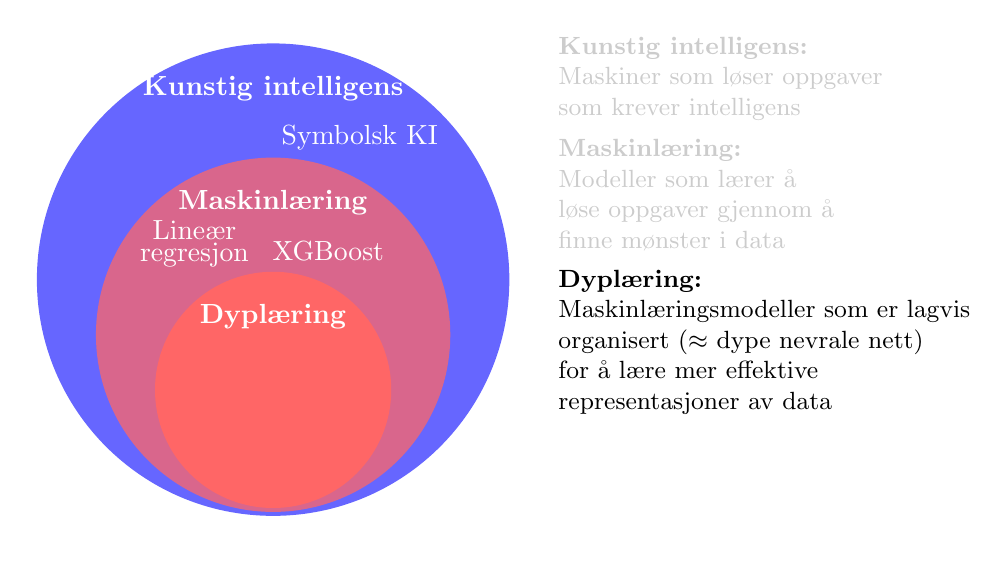
\begin{tikzpicture}
			\node[circle, fill=blue!60, minimum size=6cm] (ai) at (0, 0) {};
			\node[text=white, anchor=north] at ($ (ai.north) - (0, 0.3) $) {\textbf{Kunstig intelligens}};
			\node[text=white] at ($ (ai.north) - (-1.1, 1.2) $) {Symbolsk KI};
			\node[circle, fill=purple!60, minimum size=4.5cm, anchor=south] (ml) at ($ (ai.south) + (0, 0.05) $) {};
			\node[text=white, anchor=north] at ($ (ml.north) - (0, 0.3) $) {\textbf{Maskinlæring}};
			\node[text=white, align=center, font=\linespread{0.5}\selectfont] at ($ (ml.north) - (1, 1.1) $) {Lineær\\regresjon};
			\node[text=white, align=center] at ($ (ml.north) - (-0.7, 1.2) $) {XGBoost};
			\node[circle, fill=red!60, minimum size=3cm, anchor=south] (dl) at ($ (ai.south) + (0, 0.1) $) {};
			\node[text=white, anchor=north] at ($ (dl.north) - (0, 0.3) $) {\textbf{Dyplæring}};
			\node[anchor=north west, align=left, font=\small, text=gray!40] (ai-text) at ($ (ai.north) + (3.5, 0.2) $) {\textbf{Kunstig intelligens:}\\Maskiner som løser oppgaver\\som krever intelligens};
			\node[anchor=north west, align=left, font=\small, text=gray!40] (ml-text) at ($ (ai-text.south west) - (0, 0) $) {\textbf{Maskinlæring:}\\Modeller som lærer å\\løse oppgaver gjennom å\\finne mønster i data};
			\node[anchor=north west, align=left, font=\small] (dl-text) at ($ (ml-text.south west) - (0, 0) $) {\textbf{Dyplæring:}\\Maskinlæringsmodeller som er lagvis\\ organisert ($\approx$ dype nevrale nett)\\for å lære mer effektive\\representasjoner av data};
			\node[] at (-3, 3) {};
			\node[] at (7.7, -3.2) {};
		\end{tikzpicture}
		\vfill
	\end{frame}

	\begin{frame}{Terminologi: Taksonomi} % Taxonomy, CNNs and LLMs
		\centering
		\vfill
		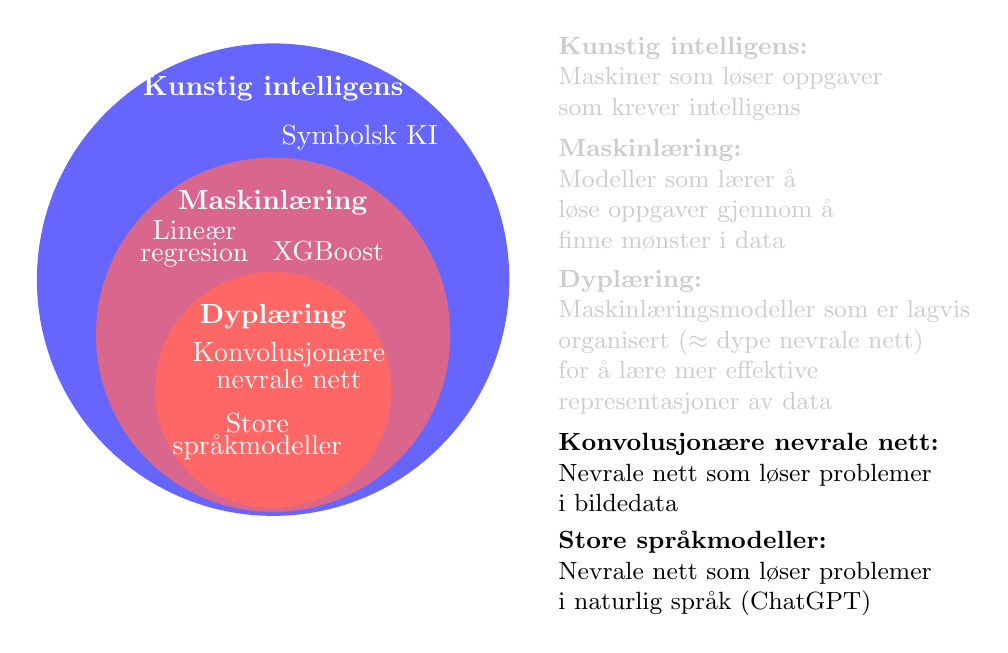
\begin{tikzpicture}
			\node[circle, fill=blue!60, minimum size=6cm] (ai) at (0, 0) {};
			\node[text=white, anchor=north] at ($ (ai.north) - (0, 0.3) $) {\textbf{Kunstig intelligens}};
			\node[text=white] at ($ (ai.north) - (-1.1, 1.2) $) {Symbolsk KI};
			\node[circle, fill=purple!60, minimum size=4.5cm, anchor=south] (ml) at ($ (ai.south) + (0, 0.05) $) {};
			\node[text=white, anchor=north] at ($ (ml.north) - (0, 0.3) $) {\textbf{Maskinlæring}};
			\node[text=white, align=center, font=\linespread{0.5}\selectfont] at ($ (ml.north) - (1, 1.1) $) {Lineær\\regresion};
			\node[text=white, align=center] at ($ (ml.north) - (-0.7, 1.2) $) {XGBoost};
			\node[circle, fill=red!60, minimum size=3cm, anchor=south] (dl) at ($ (ai.south) + (0, 0.1) $) {};
			\node[text=white, anchor=north] at ($ (dl.north) - (0, 0.3) $) {\textbf{Dyplæring}};
			\node[align=center, text=white, font=\linespread{0.5}\selectfont] at ($ (dl.north) - (-0.2, 1.2) $) {Konvolusjonære\\nevrale nett};
			\node[align=center, text=white, font=\linespread{0.5}\selectfont] at ($ (dl.north) - (0.2, 2.1) $) {Store\\språkmodeller};
			\node[anchor=north west, align=left, font=\small, text=gray!40] (ai-text) at ($ (ai.north) + (3.5, 0.2) $) {\textbf{Kunstig intelligens:}\\Maskiner som løser oppgaver\\som krever intelligens};
			\node[anchor=north west, align=left, font=\small, text=gray!40] (ml-text) at ($ (ai-text.south west) - (0, 0) $) {\textbf{Maskinlæring:}\\Modeller som lærer å\\løse oppgaver gjennom å\\finne mønster i data};
			\node[anchor=north west, align=left, font=\small, text=gray!40] (dl-text) at ($ (ml-text.south west) - (0, 0) $) {\textbf{Dyplæring:}\\Maskinlæringsmodeller som er lagvis\\ organisert ($\approx$ dype nevrale nett)\\for å lære mer effektive\\representasjoner av data};
			\node[anchor=north west, align=left, font=\small] (cnn-text) at ($ (dl-text.south west) - (0, 0) $) {\textbf{Konvolusjonære nevrale nett:}\\Nevrale nett som løser problemer\\i bildedata};
			\node[anchor=north west, align=left, font=\small] at ($ (cnn-text.south west) - (0, 0) $) {\textbf{Store språkmodeller:}\\Nevrale nett som løser problemer\\i naturlig språk (ChatGPT)};
			\node[] at (-3, 3) {};
			\node[] at (7.7, -3.2) {};
		\end{tikzpicture}
		\vfill
	\end{frame}

	\begin{frame}{Terminologi: Sterk vs svak KI} % Strong vs weak, axis
		\centering
		\vfill
		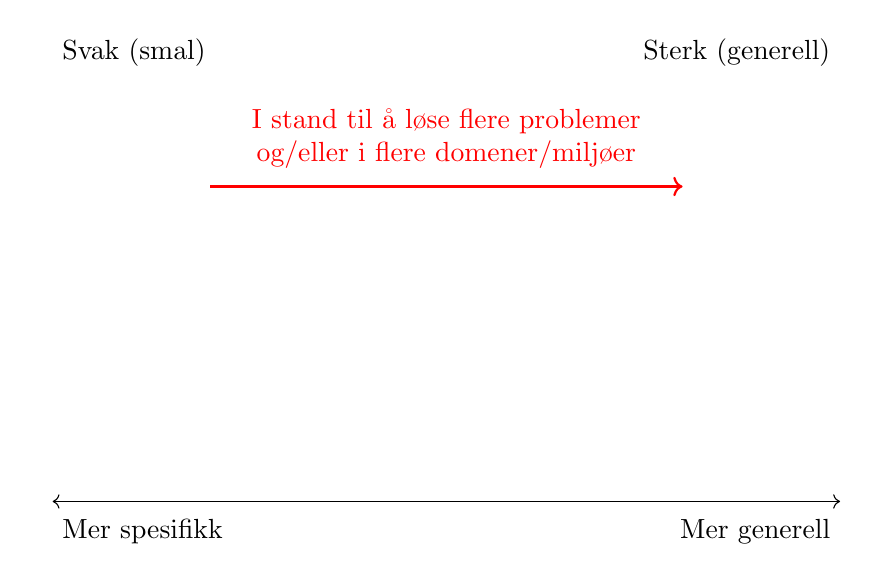
\begin{tikzpicture}
			\draw[<->] (0, 0) -- (10, 0);
			\node[anchor=north west] at (0, -0.1) {Mer spesifikk};
			\node[anchor=north east] at (10, -0.1) {Mer generell};
			\node[anchor=north west] at (0, 6) {Svak (smal)};
			\node[anchor=north east] at (10, 6) {Sterk (generell)};

			\draw[red, ->, thick] (2, 4) -- (8, 4);
			\node[anchor=south,align=center,text=red] at (5, 4.1) {I stand til å løse flere problemer\\og/eller i flere domener/miljøer};

			\node[] at (10.2, -0.4) {};
			\node[] at (-0.2, 5.9) {};
		\end{tikzpicture}
		\vfill
	\end{frame}

	\begin{frame}{Terminologi: Sterk vs svak KI} % Strong vs weak, dichotomi
		\centering
		\vfill
		\begin{tikzpicture}
			\draw[<->] (0, 0) -- (10, 0);
			\node[anchor=north west] at (0, -0.1) {Mer spesifikk};
			\node[anchor=north east] at (10, -0.1) {Mer generell};
			\node[anchor=north west] at (0, 6) {Svak (smal)};
			\node[anchor=north east] at (10, 6) {Sterk (generell)};

			\draw[red, ->, thick] (2, 4) -- (8, 4);
			\node[anchor=south,align=center,text=red] at (5, 4.1) {I stand til å løse flere problemer\\og/eller i flere domener/miljøer};
			\node[anchor=south east] at (9.5, 0.2) {
				\includegraphics[width=1.3cm]{data/human.png}
			};
			\node[anchor=south west] at (0.5, 0.2) {
				\includegraphics[width=1.3cm]{data/laptop.png}
			};
			\node[] at (10.2, -0.4) {};
			\node[] at (-0.2, 5.9) {};
		\end{tikzpicture}
		\vfill
	\end{frame}

	\begin{frame}{Terminologi: Sterk vs svak KI} % Strong vs weak, weak
		\centering
		\vfill
		\begin{tikzpicture}
			\draw[<->] (0, 0) -- (10, 0);
			\node[anchor=north west] at (0, -0.1) {Mer spesifikk};
			\node[anchor=north east] at (10, -0.1) {Mer generell};
			\node[anchor=north west] at (0, 6) {Svak (smal)};
			\node[anchor=north east] at (10, 6) {Sterk (generell)};

			\draw[red, ->, thick] (2, 4) -- (8, 4);
			\node[anchor=south,align=center,text=red] at (5, 4.1) {I stand til å løse flere problemer\\og/eller i flere domener/miljøer};
			\node[anchor=south east] at (9.5, 0.2) {
				\includegraphics[width=1.3cm]{data/human.png}
			};
			\node[anchor=south west] at (0.5, 0.2) {
				\includegraphics[width=1.3cm]{data/laptop.png}
			};
			\node[align=center,font=\small, fill=blue!60, text=white, minimum width=1.6cm, rounded corners=.1cm] at (3, 2.1) {
				Bilde-\\
				diagnostikk
			};
			\node[align=center,font=\small, fill=blue!60, text=white, minimum width=1.6cm, rounded corners=.1cm] at (3, 1.3) {
				Forsikrings-\\
				prising
			};
			\node[align=center,font=\small, fill=blue!60, text=white, minimum width=1.6cm, rounded corners=.1cm] at (3, 0.5) {
				Dokument-\\
				lesing
			};
			\node[] at (10.2, -0.4) {};
			\node[] at (-0.2, 5.9) {};
		\end{tikzpicture}
		\vfill
	\end{frame}

	\begin{frame}{Terminologi: Sterk vs svak KI} % Strong vs weak, stronger
		\centering
		\vfill
		\begin{tikzpicture}
			\draw[<->] (0, 0) -- (10, 0);
			\node[anchor=north west] at (0, -0.1) {Mer spesifikk};
			\node[anchor=north east] at (10, -0.1) {Mer generell};
			\node[anchor=north west] at (0, 6) {Svak (smal)};
			\node[anchor=north east] at (10, 6) {Sterk (generell)};

			\draw[red, ->, thick] (2, 4) -- (8, 4);
			\node[anchor=south,align=center,text=red] at (5, 4.1) {I stand til å løse flere problemer\\og/eller i flere domener/miljøer};
			\node[anchor=south east] at (9.5, 0.2) {
				\includegraphics[width=1.3cm]{data/human.png}
			};
			\node[anchor=south west] at (0.5, 0.2) {
				\includegraphics[width=1.3cm]{data/laptop.png}
			};
			\node[align=center,font=\small, fill=blue!60, text=white, minimum width=1.6cm, rounded corners=.1cm] at (3, 2.1) {
				Bilde-\\
				diagnostikk
			};
			\node[align=center,font=\small, fill=blue!60, text=white, minimum width=1.6cm, rounded corners=.1cm] at (3, 1.3) {
				Forsikrings-\\
				prising
			};
			\node[align=center,font=\small, fill=blue!60, text=white, minimum width=1.6cm, rounded corners=.1cm] at (3, 0.5) {
				Dokument-\\
				lesing
			};
			\node[align=center,font=\small, fill=blue!60, text=white, minimum width=1.6cm, rounded corners=.1cm] at (4.8, 0.5) {
				Tesla
			};
			\node[align=center,font=\small, fill=blue!60, text=white, minimum width=1.6cm, rounded corners=.1cm] at (5.4, 1.1) {
				ChatGPT
			};
			\node[] at (10.2, -0.4) {};
			\node[] at (-0.2, 5.9) {};
		\end{tikzpicture}
		\vfill
	\end{frame}

	\begin{frame}{Terminologi: Veiledet vs ikke-veiledet læring} % Supervised vs unsupervised
		\centering
		\vfill
		\begin{tikzpicture}
			\node[align=center, anchor=north] (supervised) at (0, 0) {Veiledet læring\\(Supervised learning)};
			\node[align=center, anchor=north] (unsupervised) at (7, 0) {Ikke-veiledet læring\\(Unsupervised learning)};
			\draw[] (3.5, 0) -- (3.5, -7.5);
			\node[] (cat1) at ($ (supervised.south) + (-1, -0.8) $) {
				\includegraphics[width=1.2cm]{data/cat.1.jpg}
			};
			\node[anchor=west] (cattext1) at ($ (cat1.east) + (1.2, 0) $) {Katt};
			\draw[->] (cat1) -- (cattext1);
			\node[anchor=north] (dog1) at ($ (cat1.south) + (0, -0.1) $) {
				\includegraphics[width=1.2cm]{data/dog.0.jpg}
			};
			\node[anchor=west] (dogtext1) at ($ (dog1.east) + (1.2, 0) $) {Hund};
			\draw[->] (dog1) -- (dogtext1);
			\node[anchor=north] (cat2) at ($ (dog1.south) + (0, -0.1) $) {
				\includegraphics[width=1.2cm]{data/cat.2.jpg}
			};
			\node[anchor=west] (cattext2) at ($ (cat2.east) + (1.2, 0) $) {Katt};
			\draw[->] (cat2) -- (cattext2);
			\node[anchor=north] (dog2) at ($ (cat2.south) + (0, -0.1) $) {
				\includegraphics[width=1.2cm]{data/dog.1.jpg}
			};
			\node[anchor=west] (dogtext2) at ($ (dog2.east) + (1.2, 0) $) {Hund};
			\draw[->] (dog2) -- (dogtext2);

			\node[] (cat1) at ($ (unsupervised.south) + (-1.2, -1.1) $) {
				\includegraphics[width=0.8cm]{data/cat.1.jpg}
			};
			\node[] (cat2) at ($ (cat1) + (-0.9, 0.2) $) {
				\includegraphics[width=0.8cm]{data/cat.2.jpg}
			};
			\node[] (cat3) at ($ (cat1) + (-0.5, -0.8) $) {
				\includegraphics[width=0.8cm]{data/cat.3.jpg}
			};
			\node[] (cat4) at ($ (cat1) + (0.9, -0.1) $) {
				\includegraphics[width=0.8cm]{data/cat.4.jpg}
			};

			\node[] (dog1) at ($ (cat1) + (1.8, -1.5) $) {
				\includegraphics[width=0.8cm]{data/dog.0.jpg}
			};
			\node[] (dog2) at ($ (dog1) + (0.9, 0.1) $) {
				\includegraphics[width=0.8cm]{data/dog.1.jpg}
			};
			\node[] (dog3) at ($ (dog1) + (0.3, -0.8) $) {
				\includegraphics[width=0.8cm]{data/dog.3.jpg}
			};
			\node[] (dog4) at ($ (dog1) + (-0.9, -0.3) $) {
				\includegraphics[width=0.8cm]{data/dog.4.jpg}
			};
			\draw[dashed, thick, red] ($ (cat1) + (-0.9, -1.7) $) -- ($ (dog1) + (1.2, 1.7) $);

			\node[
				fill=gray!10,
				draw=black,
				rounded corners=.1cm,
				minimum width=5cm,
				text depth=0.1cm,
				align=center,
				font=\linespread{2.5}\selectfont
			] at ($ (unsupervised.south) + (-1.4, -5) $) {
				\textbf{Generative modeller}\\
				Oslo er hovedstaden i \uline{\hspace{5em}}
			};
		\end{tikzpicture}
		\vfill
	\end{frame}

	\begin{frame}{Teori: Data} % Housing data
		\centering
		\vfill
		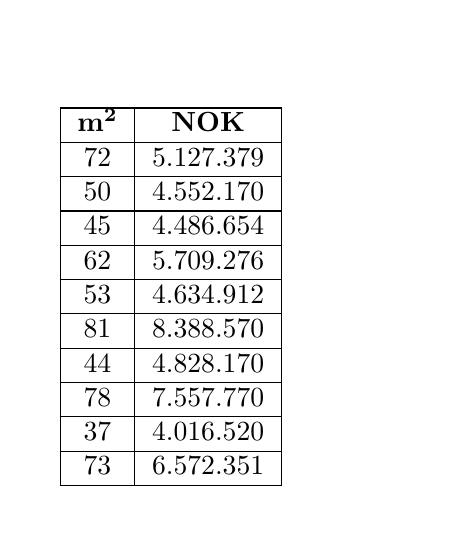
\begin{tikzpicture}
			\node[] at (0, 0) {
				\begin{tabular}{|c|c|}
					\hline
					$\mathbf{m^2}$&\textbf{NOK}\\
					\hline
					72&5.127.379\\
					\hline
					50&4.552.170\\
					\hline
					45&4.486.654\\
					\hline
					62&5.709.276\\
					\hline
					53&4.634.912\\
					\hline
					81&8.388.570\\
					\hline
					44&4.828.170\\
					\hline
					78&7.557.770\\
					\hline
					37&4.016.520\\
					\hline
					73&6.572.351\\
					\hline
				\end{tabular}
			};
			\node[] at (-1.7, 3.3) {};
			\node[] at (3.2, -2.6) {};
		\end{tikzpicture}
		\vfill
	\end{frame}

	\begin{frame}{Teori: Data} % Terminology
		\centering
		\vfill
		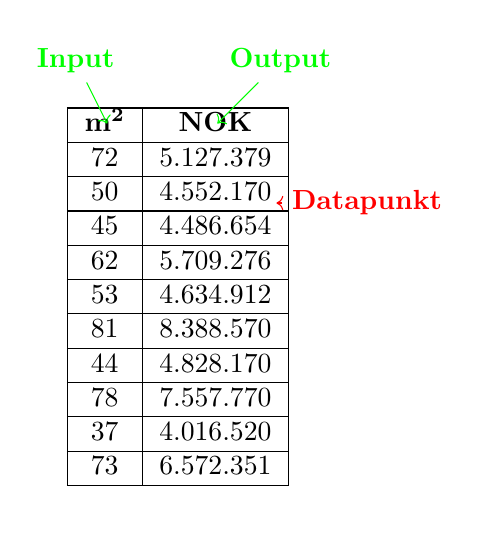
\begin{tikzpicture}
			\node[] at (0, 0) {
				\begin{tabular}{|c|c|}
					\hline
					$\mathbf{m^2}$&\textbf{NOK}\\
					\hline
					72&5.127.379\\
					\hline
					50&4.552.170\\
					\hline
					45&4.486.654\\
					\hline
					62&5.709.276\\
					\hline
					53&4.634.912\\
					\hline
					81&8.388.570\\
					\hline
					44&4.828.170\\
					\hline
					78&7.557.770\\
					\hline
					37&4.016.520\\
					\hline
					73&6.572.351\\
					\hline
				\end{tabular}
			};
			\node[] (input) at (-1.3, 3) {
				\textcolor{green}{\textbf{Input}}
			};
			\draw[->, green] (input) -- (-0.9, 2.2);
			\node[] (output) at (1.3, 3) {
				\textcolor{green}{\textbf{Output}}
			};
			\draw[->, green] (output) -- (0.5, 2.2);
			\node[] (datapoint) at (2.4, 1.19) {
				\textcolor{red}{\textbf{Datapunkt}}
			};
			\draw[->, red] (datapoint) -- (1.25, 1.19);
			\node[] at (-1.7, 3.3) {};
			\node[] at (3.2, -2.6) {};
		\end{tikzpicture}
		\vfill
	\end{frame}

	\begin{frame}{Teori: Data} % 2d dataset
		\vfill
		\centering
		\begin{tikzpicture}
			\begin{axis}[
				xlabel=$m^2$,
				ylabel=NOK,
				ytick={4000000, 5000000, 6000000, 7000000, 8000000},
				yticklabels={4M, 5M, 6M, 7M, 8M},
				scaled y ticks=false,
				xtick pos=bottom,
				ytick pos=left,
				xmin=30,
				xmax=90,,
				ymin=3500000,
				ymax=8800000,
				height=5cm,
				width=8cm
			]
				\addplot[
					only marks,
					mark size=3pt,
					mark options={draw=black, fill=cyan}
				] coordinates {
					(72, 5127379)
					(50, 4552170)
					(45, 4486654)
					(62, 5709276)
					(53, 4634912)
					(81, 8388570)
					(44, 4828170)
					(78, 7557770)
					(37, 4016520)
					(73, 6572351)
				};

				\newcommand{\loss}[2]{
					\addplot[dashed] coordinates {
						(####1, 3500000 + ####1 * 30000)
						(####1, ####2)
					};
				}

				\coordinate (center) at (axis cs: 60, 3500000);
			\end{axis}

			\node[] at ($ (center) - (4.1, -3.5) $) {};
			\node[] at ($ (center) + (4.1, -3.5) $) {};
		\end{tikzpicture}
		\vfill
	\end{frame}

	\begin{frame}{Teori: Modeller} % General model
		\vfill
		\centering
		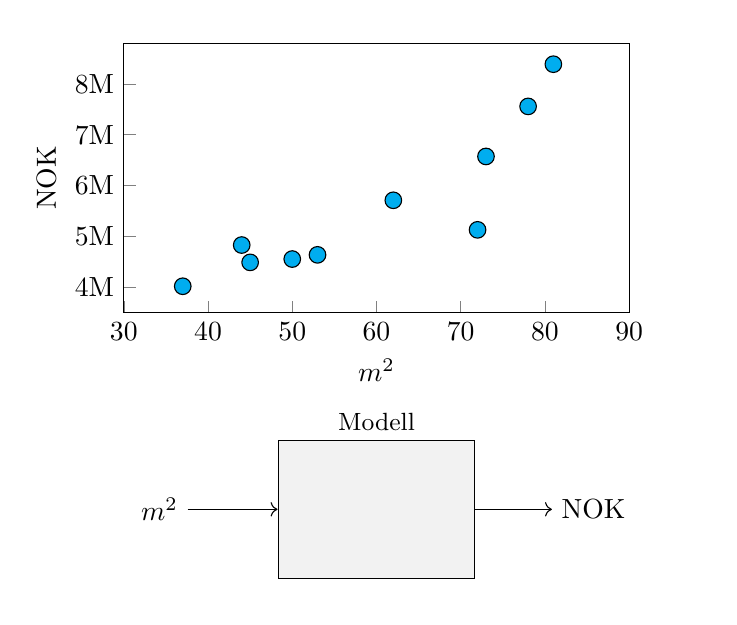
\begin{tikzpicture}
			\begin{axis}[
				xlabel=$m^2$,
				ylabel=NOK,
				ytick={4000000, 5000000, 6000000, 7000000, 8000000},
				yticklabels={4M, 5M, 6M, 7M, 8M},
				scaled y ticks=false,
				xtick pos=bottom,
				ytick pos=left,
				xmin=30,
				xmax=90,,
				ymin=3500000,
				ymax=8800000,
				height=5cm,
				width=8cm
			]
				\addplot[
					only marks,
					mark size=3pt,
					mark options={draw=black, fill=cyan}
				] coordinates {
					(72, 5127379)
					(50, 4552170)
					(45, 4486654)
					(62, 5709276)
					(53, 4634912)
					(81, 8388570)
					(44, 4828170)
					(78, 7557770)
					(37, 4016520)
					(73, 6572351)
				};
				\coordinate (center) at (axis cs: 60, 3500000);
			\end{axis}

			\node[
				draw=black,
				minimum width=2.5cm,
				minimum height=1.75cm,
				fill=gray!10,
				label=\small{Modell}
			] (model) at ($ (center) - (0, 2.5) $) {};
			\node[] (input) at ($ (model.west) - (1.5, 0) $) {$m^2$};
			\node[] (output) at ($ (model.east) + (1.5, 0) $) {NOK};
			\draw[->] (input) -- (model);
			\draw[->] (model) -- (output);
			\node[] at ($ (center) - (4.1, -3.5) $) {};
			\node[] at ($ (center) + (4.1, -3.5) $) {};
		\end{tikzpicture}
		\vfill
	\end{frame}

	\begin{frame}{Teori: Modeller} % Linear model
		\vfill
		\centering
		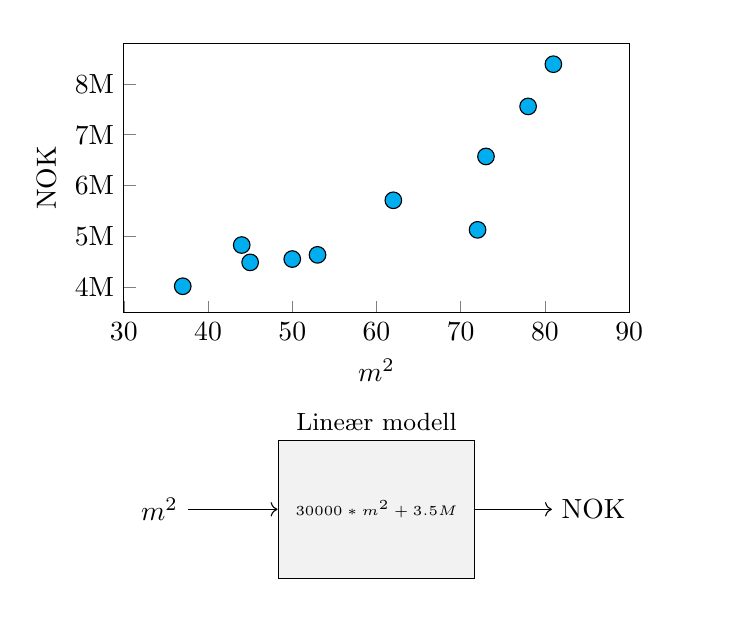
\begin{tikzpicture}
			\begin{axis}[
				xlabel=$m^2$,
				ylabel=NOK,
				ytick={4000000, 5000000, 6000000, 7000000, 8000000},
				yticklabels={4M, 5M, 6M, 7M, 8M},
				scaled y ticks=false,
				xtick pos=bottom,
				ytick pos=left,
				xmin=30,
				xmax=90,,
				ymin=3500000,
				ymax=8800000,
				height=5cm,
				width=8cm
			]
				\addplot[
					only marks,
					mark size=3pt,
					mark options={draw=black, fill=cyan}
				] coordinates {
					(72, 5127379)
					(50, 4552170)
					(45, 4486654)
					(62, 5709276)
					(53, 4634912)
					(81, 8388570)
					(44, 4828170)
					(78, 7557770)
					(37, 4016520)
					(73, 6572351)
				};
				\coordinate (center) at (axis cs: 60, 3500000);
			\end{axis}

			\node[
				draw=black,
				minimum width=2.5cm,
				minimum height=1.75cm,
				fill=gray!10,
				label=\small{Lineær modell}
			] (model) at ($ (center) - (0, 2.5) $) {\tiny{$30000*m^2+3.5M$}};
			\node[] (input) at ($ (model.west) - (1.5, 0) $) {$m^2$};
			\node[] (output) at ($ (model.east) + (1.5, 0) $) {NOK};
			\draw[->] (input) -- (model);
			\draw[->] (model) -- (output);
			\node[] at ($ (center) - (4.1, -3.5) $) {};
			\node[] at ($ (center) + (4.1, -3.5) $) {};
		\end{tikzpicture}
		\vfill
	\end{frame}

	\begin{frame}{Teori: Modeller} % Visual linear regression
		\vfill
		\centering
		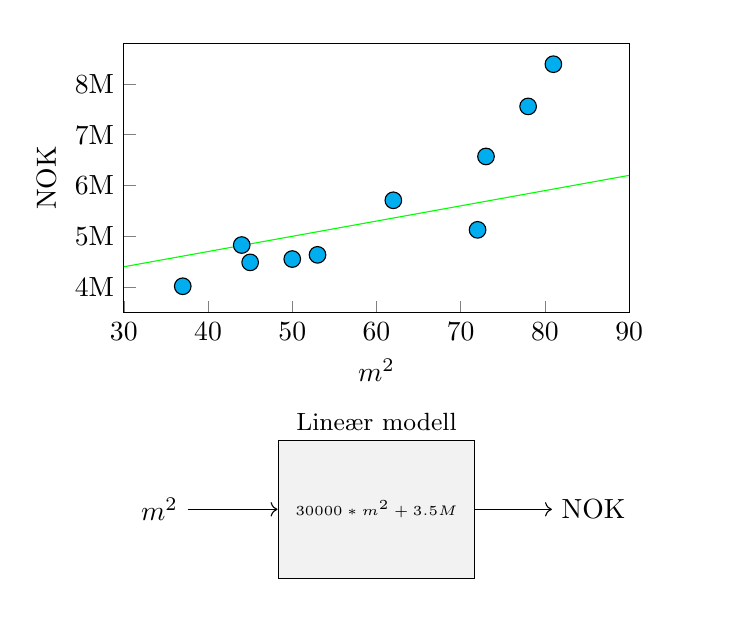
\begin{tikzpicture}
			\begin{axis}[
				xlabel=$m^2$,
				ylabel=NOK,
				ytick={4000000, 5000000, 6000000, 7000000, 8000000},
				yticklabels={4M, 5M, 6M, 7M, 8M},
				scaled y ticks=false,
				xtick pos=bottom,
				ytick pos=left,
				xmin=30,
				xmax=90,,
				ymin=3500000,
				ymax=8800000,
				height=5cm,
				width=8cm
			]
				\addplot[
					only marks,
					mark size=3pt,
					mark options={draw=black, fill=cyan}
				] coordinates {
					(72, 5127379)
					(50, 4552170)
					(45, 4486654)
					(62, 5709276)
					(53, 4634912)
					(81, 8388570)
					(44, 4828170)
					(78, 7557770)
					(37, 4016520)
					(73, 6572351)
				};
				\addplot[green] coordinates {
					(0, 3500000)
					(100, 6500000)
				};
				\coordinate (center) at (axis cs: 60, 3500000);
			\end{axis}

			\node[
				draw=black,
				minimum width=2.5cm,
				minimum height=1.75cm,
				fill=gray!10,
				label=\small{Lineær modell}
			] (model) at ($ (center) - (0, 2.5) $) {\tiny{$30000*m^2+3.5M$}};
			\node[] (input) at ($ (model.west) - (1.5, 0) $) {$m^2$};
			\node[] (output) at ($ (model.east) + (1.5, 0) $) {NOK};
			\draw[->] (input) -- (model);
			\draw[->] (model) -- (output);
			\node[] at ($ (center) - (4.1, -3.5) $) {};
			\node[] at ($ (center) + (4.1, -3.5) $) {};
		\end{tikzpicture}
		\vfill
	\end{frame}

	\begin{frame}{Teori: Prediksjon} % Prediction
		\vfill
		\centering
		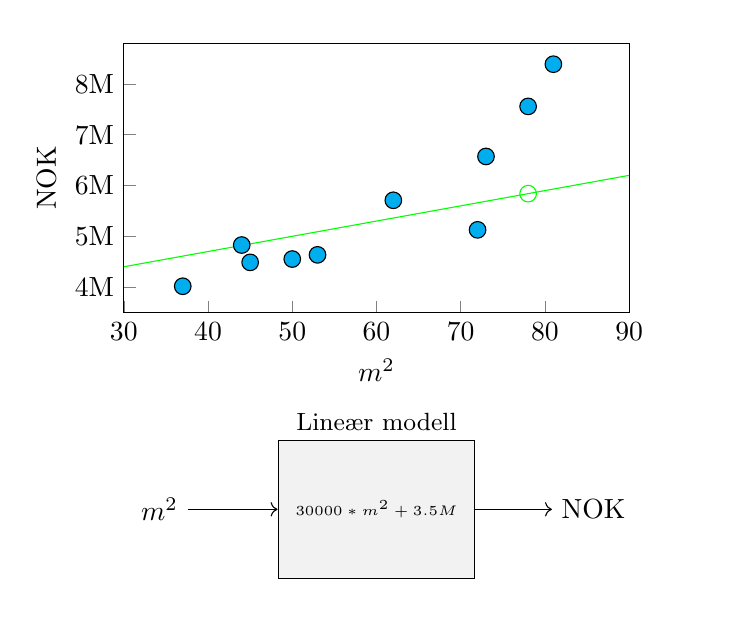
\begin{tikzpicture}
			\begin{axis}[
				xlabel=$m^2$,
				ylabel=NOK,
				ytick={4000000, 5000000, 6000000, 7000000, 8000000},
				yticklabels={4M, 5M, 6M, 7M, 8M},
				scaled y ticks=false,
				xtick pos=bottom,
				ytick pos=left,
				xmin=30,
				xmax=90,,
				ymin=3500000,
				ymax=8800000,
				height=5cm,
				width=8cm
			]
				\addplot[
					only marks,
					mark size=3pt,
					mark options={draw=black, fill=cyan}
				] coordinates {
					(72, 5127379)
					(50, 4552170)
					(45, 4486654)
					(62, 5709276)
					(53, 4634912)
					(81, 8388570)
					(44, 4828170)
					(78, 7557770)
					(37, 4016520)
					(73, 6572351)
				};
				\addplot[green] coordinates {
					(0, 3500000)
					(100, 6500000)
				};
				\addplot[
					only marks,
					mark size=3pt,
					mark options={draw=green, fill=white},
					fill opacity=0
				] coordinates {
					(78, 3500000 + 78 * 30000)
				};
				\coordinate (center) at (axis cs: 60, 3500000);
			\end{axis}

			\node[
				draw=black,
				minimum width=2.5cm,
				minimum height=1.75cm,
				fill=gray!10,
				label=\small{Lineær modell}
			] (model) at ($ (center) - (0, 2.5) $) {\tiny{$30000*m^2+3.5M$}};
			\node[] (input) at ($ (model.west) - (1.5, 0) $) {$m^2$};
			\node[] (output) at ($ (model.east) + (1.5, 0) $) {NOK};
			\draw[->] (input) -- (model);
			\draw[->] (model) -- (output);
			\node[] at ($ (center) - (4.1, -3.5) $) {};
			\node[] at ($ (center) + (4.1, -3.5) $) {};
		\end{tikzpicture}
		\vfill
	\end{frame}

	\begin{frame}{Teori: Kost} % Loss
		\vfill
		\centering
		\begin{tikzpicture}
			\begin{axis}[
				xlabel=$m^2$,
				ylabel=NOK,
				ytick={4000000, 5000000, 6000000, 7000000, 8000000},
				yticklabels={4M, 5M, 6M, 7M, 8M},
				scaled y ticks=false,
				xtick pos=bottom,
				ytick pos=left,
				xmin=30,
				xmax=90,,
				ymin=3500000,
				ymax=8800000,
				height=5cm,
				width=8cm
			]
				\addplot[
					only marks,
					mark size=3pt,
					mark options={draw=black, fill=cyan}
				] coordinates {
					(72, 5127379)
					(50, 4552170)
					(45, 4486654)
					(62, 5709276)
					(53, 4634912)
					(81, 8388570)
					(44, 4828170)
					(78, 7557770)
					(37, 4016520)
					(73, 6572351)
				};
				\addplot[green] coordinates {
					(0, 3500000)
					(100, 6500000)
				};
				\addplot[
					only marks,
					mark size=3pt,
					mark options={draw=green, fill=white},
					fill opacity=0
				] coordinates {
					(78, 3500000 + 78 * 30000)
				};


				\newcommand{\loss}[2]{
					\addplot[dashed] coordinates {
						(####1, 3500000 + ####1 * 30000)
						(####1, ####2)
					};
				}

				\loss{78}{7557770}

				\coordinate (center) at (axis cs: 60, 3500000);
			\end{axis}

			\node[
				draw=black,
				minimum width=2.5cm,
				minimum height=1.75cm,
				fill=gray!10,
				label=\small{Lineær modell}
			] (model) at ($ (center) - (0, 2.5) $) {\tiny{$30000*m^2+3.5M$}};
			\node[] (input) at ($ (model.west) - (1.5, 0) $) {$m^2$};
			\node[] (output) at ($ (model.east) + (1.5, 0) $) {NOK};
			\draw[->] (input) -- (model);
			\draw[->] (model) -- (output);
			\node[] at ($ (center) - (4.1, -3.5) $) {};
			\node[] at ($ (center) + (4.1, -3.5) $) {};
		\end{tikzpicture}
		\vfill
	\end{frame}

	\begin{frame}{Teori: Kost} % Total loss
		\vfill
		\centering
		\begin{tikzpicture}
			\begin{axis}[
				xlabel=$m^2$,
				ylabel=NOK,
				ytick={4000000, 5000000, 6000000, 7000000, 8000000},
				yticklabels={4M, 5M, 6M, 7M, 8M},
				scaled y ticks=false,
				xtick pos=bottom,
				ytick pos=left,
				xmin=30,
				xmax=90,,
				ymin=3500000,
				ymax=8800000,
				height=5cm,
				width=8cm
			]
				\addplot[
					only marks,
					mark size=3pt,
					mark options={draw=black, fill=cyan}
				] coordinates {
					(72, 5127379)
					(50, 4552170)
					(45, 4486654)
					(62, 5709276)
					(53, 4634912)
					(81, 8388570)
					(44, 4828170)
					(78, 7557770)
					(37, 4016520)
					(73, 6572351)
				};
				\addplot[green] coordinates {
					(0, 3500000)
					(100, 6500000)
				};
				\addplot[
					only marks,
					mark size=3pt,
					mark options={draw=green, fill=white},
					fill opacity=0
				] coordinates {
					(72, 3500000 + 72 * 30000)
					(50, 3500000 + 50 * 30000)
					(45, 3500000 + 45 * 30000)
					(62, 3500000 + 62 * 30000)
					(53, 3500000 + 53 * 30000)
					(81, 3500000 + 81 * 30000)
					(44, 3500000 + 44 * 30000)
					(78, 3500000 + 78 * 30000)
					(37, 3500000 + 37 * 30000)
					(73, 3500000 + 73 * 30000)
				};


				\newcommand{\loss}[2]{
					\addplot[dashed] coordinates {
						(####1, 3500000 + ####1 * 30000)
						(####1, ####2)
					};
				}

				\loss{72}{5127379}
				\loss{50}{4552170}
				\loss{45}{4486654}
				\loss{62}{5709276}
				\loss{53}{4634912}
				\loss{81}{8388570}
				\loss{44}{4828170}
				\loss{78}{7557770}
				\loss{37}{4016520}
				\loss{73}{6572351}

				\coordinate (center) at (axis cs: 60, 3500000);
			\end{axis}

			\node[
				draw=black,
				minimum width=2.5cm,
				minimum height=1.75cm,
				fill=gray!10,
				label=\small{Lineær modell}
			] (model) at ($ (center) - (0, 2.5) $) {\tiny{$30000*m^2+3.5M$}};
			\node[] (input) at ($ (model.west) - (1.5, 0) $) {$m^2$};
			\node[] (output) at ($ (model.east) + (1.5, 0) $) {NOK};
			\draw[->] (input) -- (model);
			\draw[->] (model) -- (output);
			\node[] at ($ (center) - (4.1, -3.5) $) {};
			\node[] at ($ (center) + (4.1, -3.5) $) {};
		\end{tikzpicture}
		\vfill
	\end{frame}

	\begin{frame}{Teori: Læring} % Gradient descent
		\vfill
		\centering
		\begin{tikzpicture}
			\begin{axis}[
				xlabel=$m^2$,
				ylabel=NOK,
				ytick={4000000, 5000000, 6000000, 7000000, 8000000},
				yticklabels={4M, 5M, 6M, 7M, 8M},
				scaled y ticks=false,
				xtick pos=bottom,
				ytick pos=left,
				xmin=30,
				xmax=90,,
				ymin=3500000,
				ymax=8800000,
				height=5cm,
				width=8cm
			]
				\addplot[
					only marks,
					mark size=3pt,
					mark options={draw=black, fill=cyan}
				] coordinates {
					(72, 5127379)
					(50, 4552170)
					(45, 4486654)
					(62, 5709276)
					(53, 4634912)
					(81, 8388570)
					(44, 4828170)
					(78, 7557770)
					(37, 4016520)
					(73, 6572351)
				};
				\addplot[green] coordinates {
					(0, 3500000)
					(100, 6500000)
				};
				\addplot[
					only marks,
					mark size=3pt,
					mark options={draw=green, fill=white},
					fill opacity=0
				] coordinates {
					(72, 3500000 + 72 * 30000)
					(50, 3500000 + 50 * 30000)
					(45, 3500000 + 45 * 30000)
					(62, 3500000 + 62 * 30000)
					(53, 3500000 + 53 * 30000)
					(81, 3500000 + 81 * 30000)
					(44, 3500000 + 44 * 30000)
					(78, 3500000 + 78 * 30000)
					(37, 3500000 + 37 * 30000)
					(73, 3500000 + 73 * 30000)
				};


				\newcommand{\loss}[2]{
					\addplot[dashed, red] coordinates {
						(####1, 3500000 + ####1 * 30000)
						(####1, ####2)
					};
				}

				\loss{72}{5127379}
				\loss{50}{4552170}
				\loss{45}{4486654}
				\loss{62}{5709276}
				\loss{53}{4634912}
				\loss{81}{8388570}
				\loss{44}{4828170}
				\loss{78}{7557770}
				\loss{37}{4016520}
				\loss{73}{6572351}

				\coordinate (center) at (axis cs: 60, 3500000);
			\end{axis}

			\node[
				draw=black,
				minimum width=2.5cm,
				minimum height=1.75cm,
				fill=gray!10,
				label=\small{Lineær modell}
			] (model) at ($ (center) - (0, 2.5) $) {\tiny{\textcolor{red}{$30000$}$*m^2+$\textcolor{red}{$3.5M$}}};
			\node[] (input) at ($ (model.west) - (1.5, 0) $) {$m^2$};
			\node[] (output) at ($ (model.east) + (1.5, 0) $) {NOK};
			\draw[->] (input) -- (model);
			\draw[->] (model) -- (output);
			\node[] at ($ (center) - (4.1, -3.5) $) {};
			\node[] at ($ (center) + (4.1, -3.5) $) {};
		\end{tikzpicture}
		\vfill
	\end{frame}

	\begin{frame}{Teori: Læring} % Update
		\vfill
		\centering
		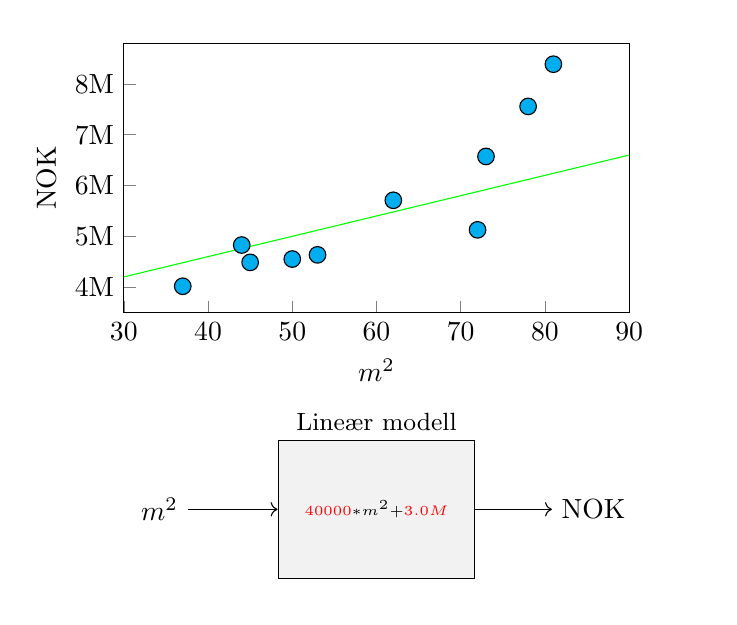
\begin{tikzpicture}
			\begin{axis}[
				xlabel=$m^2$,
				ylabel=NOK,
				ytick={4000000, 5000000, 6000000, 7000000, 8000000},
				yticklabels={4M, 5M, 6M, 7M, 8M},
				scaled y ticks=false,
				xtick pos=bottom,
				ytick pos=left,
				xmin=30,
				xmax=90,,
				ymin=3500000,
				ymax=8800000,
				height=5cm,
				width=8cm
			]
				\addplot[
					only marks,
					mark size=3pt,
					mark options={draw=black, fill=cyan}
				] coordinates {
					(72, 5127379)
					(50, 4552170)
					(45, 4486654)
					(62, 5709276)
					(53, 4634912)
					(81, 8388570)
					(44, 4828170)
					(78, 7557770)
					(37, 4016520)
					(73, 6572351)
				};
				\addplot[green] coordinates {
					(0, 3000000)
					(100, 7000000)
				};

				\newcommand{\loss}[2]{
					\addplot[dashed, red] coordinates {
						(####1, 3500000 + ####1 * 30000)
						(####1, ####2)
					};
				}

				\coordinate (center) at (axis cs: 60, 3500000);
			\end{axis}

			\node[
				draw=black,
				minimum width=2.5cm,
				minimum height=1.75cm,
				fill=gray!10,
				label=\small{Lineær modell}
			] (model) at ($ (center) - (0, 2.5) $) {\tiny{\textcolor{red}{$40000$}$*m^2+$\textcolor{red}{$3.0M$}}};
			\node[] (input) at ($ (model.west) - (1.5, 0) $) {$m^2$};
			\node[] (output) at ($ (model.east) + (1.5, 0) $) {NOK};
			\draw[->] (input) -- (model);
			\draw[->] (model) -- (output);
			\node[] at ($ (center) - (4.1, -3.5) $) {};
			\node[] at ($ (center) + (4.1, -3.5) $) {};
		\end{tikzpicture}
		\vfill
	\end{frame}

	\begin{frame}{Teori: Nevrale nett} % Neural net
		\vfill
		\centering
		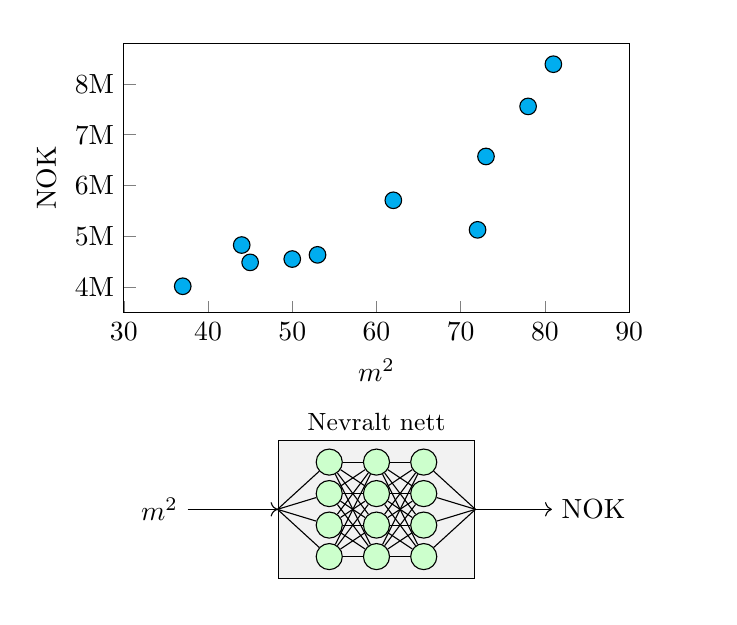
\begin{tikzpicture}
			\begin{axis}[
				xlabel=$m^2$,
				ylabel=NOK,
				ytick={4000000, 5000000, 6000000, 7000000, 8000000},
				yticklabels={4M, 5M, 6M, 7M, 8M},
				scaled y ticks=false,
				xtick pos=bottom,
				ytick pos=left,
				xmin=30,
				xmax=90,,
				ymin=3500000,
				ymax=8800000,
				height=5cm,
				width=8cm
			]
				\addplot[
					only marks,
					mark size=3pt,
					mark options={draw=black, fill=cyan}
				] coordinates {
					(72, 5127379)
					(50, 4552170)
					(45, 4486654)
					(62, 5709276)
					(53, 4634912)
					(81, 8388570)
					(44, 4828170)
					(78, 7557770)
					(37, 4016520)
					(73, 6572351)
				};

				\newcommand{\loss}[2]{
					\addplot[dashed, red] coordinates {
						(####1, 3500000 + ####1 * 30000)
						(####1, ####2)
					};
				}

				\coordinate (center) at (axis cs: 60, 3500000);
			\end{axis}

			\node[
				draw=black,
				minimum width=2.5cm,
				minimum height=1.75cm,
				fill=gray!10,
				label=\small{Nevralt nett}
			] (model) at ($ (center) - (0, 2.5) $) {};
			\node[] (input) at ($ (model.west) - (1.5, 0) $) {$m^2$};
			\node[] (output) at ($ (model.east) + (1.5, 0) $) {NOK};
			\draw[->] (input) -- (model);
			\draw[->] (model) -- (output);
			\node[] at ($ (center) - (4.1, -3.5) $) {};
			\node[] at ($ (center) + (4.1, -3.5) $) {};
			\node[circle, draw=black, fill=green!20] (n11) at ($ (model) + (0, 0.2) $) {};
			\node[circle, draw=black, fill=green!20] (n12) at ($ (model) + (0, -0.2) $) {};
			\node[circle, draw=black, fill=green!20] (n10) at ($ (model) + (0, 0.6) $) {};
			\node[circle, draw=black, fill=green!20] (n13) at ($ (model) + (0, -0.6) $) {};

			\node[circle, draw=black, fill=green!20] (n01) at ($ (model) + (-0.6, 0.2) $) {};
			\node[circle, draw=black, fill=green!20] (n02) at ($ (model) + (-0.6, -0.2) $) {};
			\node[circle, draw=black, fill=green!20] (n00) at ($ (model) + (-0.6, 0.6) $) {};
			\node[circle, draw=black, fill=green!20] (n03) at ($ (model) + (-0.6, -0.6) $) {};


			\node[circle, draw=black, fill=green!20] (n21) at ($ (model) + (0.6, 0.2) $) {};
			\node[circle, draw=black, fill=green!20] (n22) at ($ (model) + (0.6, -0.2) $) {};
			\node[circle, draw=black, fill=green!20] (n20) at ($ (model) + (0.6, 0.6) $) {};
			\node[circle, draw=black, fill=green!20] (n23) at ($ (model) + (0.6, -0.6) $) {};

			\draw[] (model.west) -- (n00);
			\draw[] (model.west) -- (n01);
			\draw[] (model.west) -- (n02);
			\draw[] (model.west) -- (n03);

			\draw[] (n00) -- (n10);
			\draw[] (n00) -- (n11);
			\draw[] (n00) -- (n12);
			\draw[] (n00) -- (n13);
			\draw[] (n01) -- (n10);
			\draw[] (n01) -- (n11);
			\draw[] (n01) -- (n12);
			\draw[] (n01) -- (n13);
			\draw[] (n02) -- (n10);
			\draw[] (n02) -- (n11);
			\draw[] (n02) -- (n12);
			\draw[] (n02) -- (n13);
			\draw[] (n03) -- (n10);
			\draw[] (n03) -- (n11);
			\draw[] (n03) -- (n12);
			\draw[] (n03) -- (n13);

			\draw[] (n10) -- (n20);
			\draw[] (n10) -- (n21);
			\draw[] (n10) -- (n22);
			\draw[] (n10) -- (n23);
			\draw[] (n11) -- (n20);
			\draw[] (n11) -- (n21);
			\draw[] (n11) -- (n22);
			\draw[] (n11) -- (n23);
			\draw[] (n12) -- (n20);
			\draw[] (n12) -- (n21);
			\draw[] (n12) -- (n22);
			\draw[] (n12) -- (n23);
			\draw[] (n13) -- (n20);
			\draw[] (n13) -- (n21);
			\draw[] (n13) -- (n22);
			\draw[] (n13) -- (n23);

			\draw[] (n20) -- (model.east);
			\draw[] (n21) -- (model.east);
			\draw[] (n22) -- (model.east);
			\draw[] (n23) -- (model.east);

		\end{tikzpicture}
		\vfill
	\end{frame}

	\begin{frame}{Teori: Nevrale nett} % Neural net representation
		\vfill
		\centering
		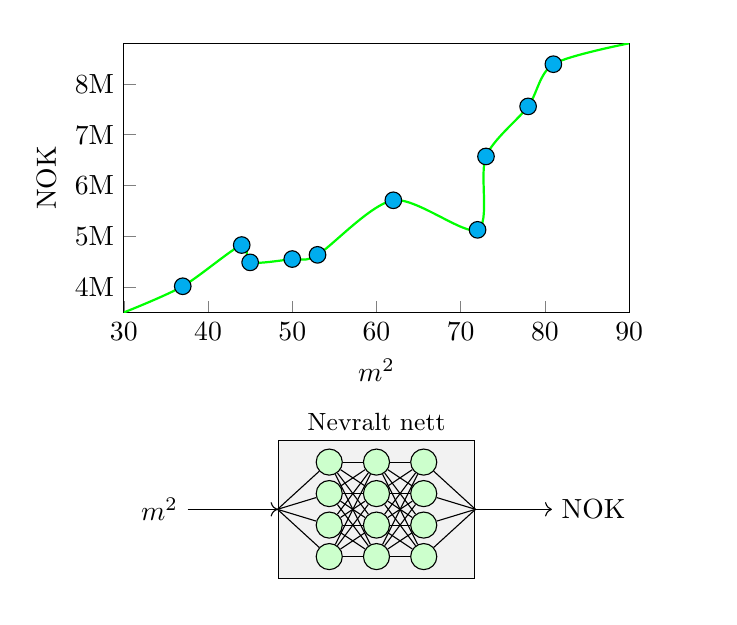
\begin{tikzpicture}
			\begin{axis}[
				xlabel=$m^2$,
				ylabel=NOK,
				ytick={4000000, 5000000, 6000000, 7000000, 8000000},
				yticklabels={4M, 5M, 6M, 7M, 8M},
				scaled y ticks=false,
				xtick pos=bottom,
				ytick pos=left,
				xmin=30,
				xmax=90,,
				ymin=3500000,
				ymax=8800000,
				height=5cm,
				width=8cm
			]
				\addplot[
					only marks,
					mark size=3pt,
					mark options={draw=black, fill=cyan}
				] coordinates {
					(72, 5127379)
					(50, 4552170)
					(45, 4486654)
					(62, 5709276)
					(53, 4634912)
					(81, 8388570)
					(44, 4828170)
					(78, 7557770)
					(37, 4016520)
					(73, 6572351)
				};
				\addplot[
					smooth,
					green,
					thick
				] coordinates {
					(30, 3500000)
					(37, 4016520)
					(44, 4828170)
					(45, 4486654)
					(50, 4552170)
					(53, 4634912)
					(62, 5709276)
					(72, 5127379)
					(73, 6572351)
					(78, 7557770)
					(81, 8388570)
					(90, 8800000)
				};

				\newcommand{\loss}[2]{
					\addplot[dashed, red] coordinates {
						(####1, 3500000 + ####1 * 30000)
						(####1, ####2)
					};
				}

				\coordinate (center) at (axis cs: 60, 3500000);
			\end{axis}

			\node[
				draw=black,
				minimum width=2.5cm,
				minimum height=1.75cm,
				fill=gray!10,
				label=\small{Nevralt nett}
			] (model) at ($ (center) - (0, 2.5) $) {};
			\node[] (input) at ($ (model.west) - (1.5, 0) $) {$m^2$};
			\node[] (output) at ($ (model.east) + (1.5, 0) $) {NOK};
			\draw[->] (input) -- (model);
			\draw[->] (model) -- (output);
			\node[] at ($ (center) - (4.1, -3.5) $) {};
			\node[] at ($ (center) + (4.1, -3.5) $) {};
			\node[circle, draw=black, fill=green!20] (n11) at ($ (model) + (0, 0.2) $) {};
			\node[circle, draw=black, fill=green!20] (n12) at ($ (model) + (0, -0.2) $) {};
			\node[circle, draw=black, fill=green!20] (n10) at ($ (model) + (0, 0.6) $) {};
			\node[circle, draw=black, fill=green!20] (n13) at ($ (model) + (0, -0.6) $) {};

			\node[circle, draw=black, fill=green!20] (n01) at ($ (model) + (-0.6, 0.2) $) {};
			\node[circle, draw=black, fill=green!20] (n02) at ($ (model) + (-0.6, -0.2) $) {};
			\node[circle, draw=black, fill=green!20] (n00) at ($ (model) + (-0.6, 0.6) $) {};
			\node[circle, draw=black, fill=green!20] (n03) at ($ (model) + (-0.6, -0.6) $) {};


			\node[circle, draw=black, fill=green!20] (n21) at ($ (model) + (0.6, 0.2) $) {};
			\node[circle, draw=black, fill=green!20] (n22) at ($ (model) + (0.6, -0.2) $) {};
			\node[circle, draw=black, fill=green!20] (n20) at ($ (model) + (0.6, 0.6) $) {};
			\node[circle, draw=black, fill=green!20] (n23) at ($ (model) + (0.6, -0.6) $) {};

			\draw[] (model.west) -- (n00);
			\draw[] (model.west) -- (n01);
			\draw[] (model.west) -- (n02);
			\draw[] (model.west) -- (n03);

			\draw[] (n00) -- (n10);
			\draw[] (n00) -- (n11);
			\draw[] (n00) -- (n12);
			\draw[] (n00) -- (n13);
			\draw[] (n01) -- (n10);
			\draw[] (n01) -- (n11);
			\draw[] (n01) -- (n12);
			\draw[] (n01) -- (n13);
			\draw[] (n02) -- (n10);
			\draw[] (n02) -- (n11);
			\draw[] (n02) -- (n12);
			\draw[] (n02) -- (n13);
			\draw[] (n03) -- (n10);
			\draw[] (n03) -- (n11);
			\draw[] (n03) -- (n12);
			\draw[] (n03) -- (n13);

			\draw[] (n10) -- (n20);
			\draw[] (n10) -- (n21);
			\draw[] (n10) -- (n22);
			\draw[] (n10) -- (n23);
			\draw[] (n11) -- (n20);
			\draw[] (n11) -- (n21);
			\draw[] (n11) -- (n22);
			\draw[] (n11) -- (n23);
			\draw[] (n12) -- (n20);
			\draw[] (n12) -- (n21);
			\draw[] (n12) -- (n22);
			\draw[] (n12) -- (n23);
			\draw[] (n13) -- (n20);
			\draw[] (n13) -- (n21);
			\draw[] (n13) -- (n22);
			\draw[] (n13) -- (n23);

			\draw[] (n20) -- (model.east);
			\draw[] (n21) -- (model.east);
			\draw[] (n22) -- (model.east);
			\draw[] (n23) -- (model.east);

		\end{tikzpicture}
		\vfill
	\end{frame}

	\begin{frame}{Teori: Univariat regresjon} % Univariate
		\vfill
		\centering
		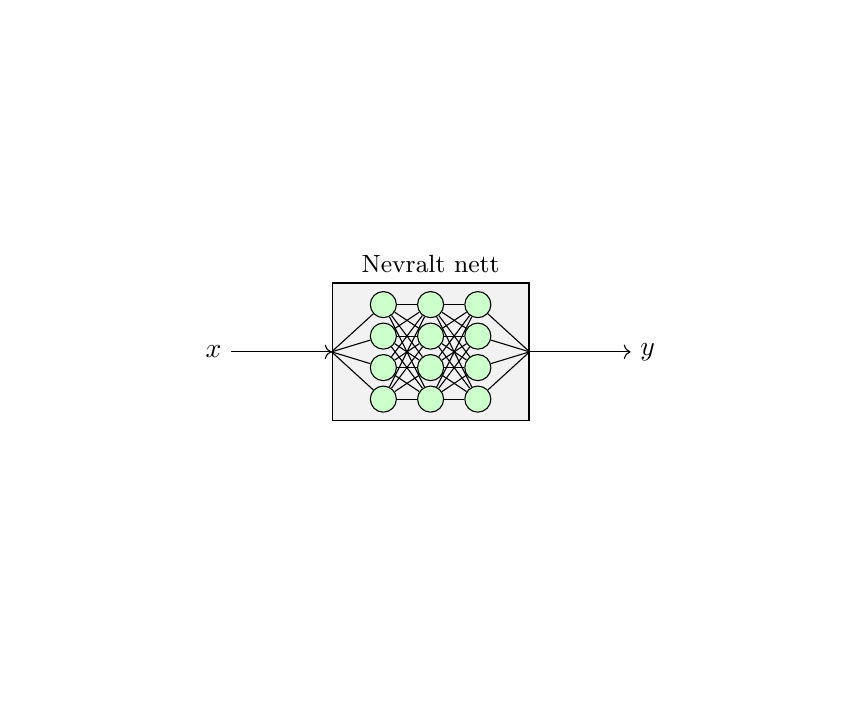
\begin{tikzpicture}
			\node[
				draw=black,
				minimum width=2.5cm,
				minimum height=1.75cm,
				fill=gray!10,
				label=\small{Nevralt nett}
			] (model) at (0, 0) {};
			\node[] (input) at ($ (model.west) - (1.5, 0) $) {$x$};
			\node[] (output) at ($ (model.east) + (1.5, 0) $) {$y$};
			\draw[->] (input) -- (model);
			\draw[->] (model) -- (output);
			\node[] at (-5, -4) {};
			\node[] at (5, 4) {};
			\node[circle, draw=black, fill=green!20] (n11) at ($ (model) + (0, 0.2) $) {};
			\node[circle, draw=black, fill=green!20] (n12) at ($ (model) + (0, -0.2) $) {};
			\node[circle, draw=black, fill=green!20] (n10) at ($ (model) + (0, 0.6) $) {};
			\node[circle, draw=black, fill=green!20] (n13) at ($ (model) + (0, -0.6) $) {};

			\node[circle, draw=black, fill=green!20] (n01) at ($ (model) + (-0.6, 0.2) $) {};
			\node[circle, draw=black, fill=green!20] (n02) at ($ (model) + (-0.6, -0.2) $) {};
			\node[circle, draw=black, fill=green!20] (n00) at ($ (model) + (-0.6, 0.6) $) {};
			\node[circle, draw=black, fill=green!20] (n03) at ($ (model) + (-0.6, -0.6) $) {};


			\node[circle, draw=black, fill=green!20] (n21) at ($ (model) + (0.6, 0.2) $) {};
			\node[circle, draw=black, fill=green!20] (n22) at ($ (model) + (0.6, -0.2) $) {};
			\node[circle, draw=black, fill=green!20] (n20) at ($ (model) + (0.6, 0.6) $) {};
			\node[circle, draw=black, fill=green!20] (n23) at ($ (model) + (0.6, -0.6) $) {};

			\draw[] (model.west) -- (n00);
			\draw[] (model.west) -- (n01);
			\draw[] (model.west) -- (n02);
			\draw[] (model.west) -- (n03);

			\draw[] (n00) -- (n10);
			\draw[] (n00) -- (n11);
			\draw[] (n00) -- (n12);
			\draw[] (n00) -- (n13);
			\draw[] (n01) -- (n10);
			\draw[] (n01) -- (n11);
			\draw[] (n01) -- (n12);
			\draw[] (n01) -- (n13);
			\draw[] (n02) -- (n10);
			\draw[] (n02) -- (n11);
			\draw[] (n02) -- (n12);
			\draw[] (n02) -- (n13);
			\draw[] (n03) -- (n10);
			\draw[] (n03) -- (n11);
			\draw[] (n03) -- (n12);
			\draw[] (n03) -- (n13);

			\draw[] (n10) -- (n20);
			\draw[] (n10) -- (n21);
			\draw[] (n10) -- (n22);
			\draw[] (n10) -- (n23);
			\draw[] (n11) -- (n20);
			\draw[] (n11) -- (n21);
			\draw[] (n11) -- (n22);
			\draw[] (n11) -- (n23);
			\draw[] (n12) -- (n20);
			\draw[] (n12) -- (n21);
			\draw[] (n12) -- (n22);
			\draw[] (n12) -- (n23);
			\draw[] (n13) -- (n20);
			\draw[] (n13) -- (n21);
			\draw[] (n13) -- (n22);
			\draw[] (n13) -- (n23);

			\draw[] (n20) -- (model.east);
			\draw[] (n21) -- (model.east);
			\draw[] (n22) -- (model.east);
			\draw[] (n23) -- (model.east);

		\end{tikzpicture}
		\vfill
	\end{frame}

	\begin{frame}{Teori: Multivariat regresjon} % Multivariate
		\vfill
		\centering
		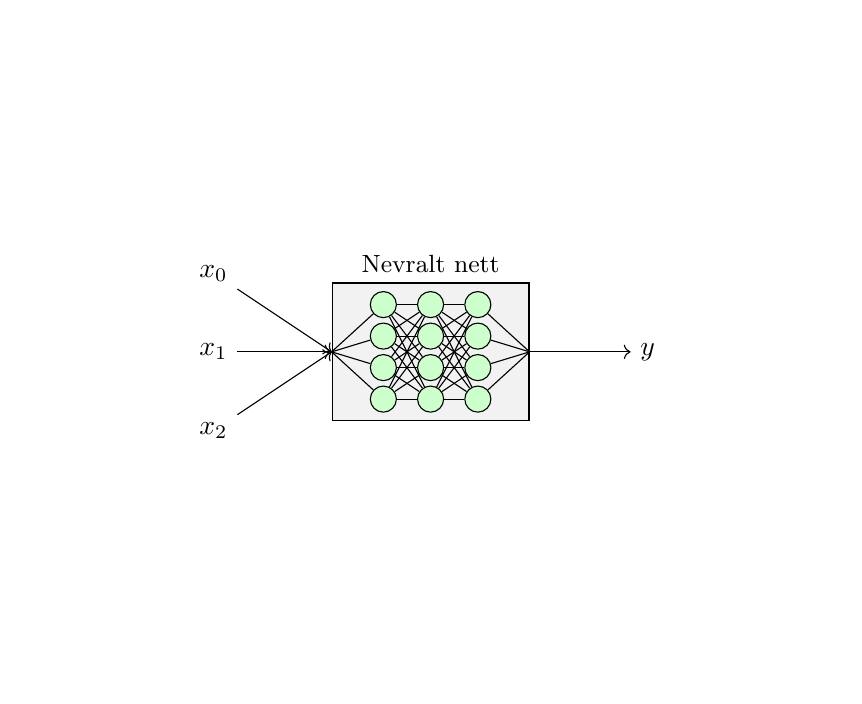
\begin{tikzpicture}
			\node[
				draw=black,
				minimum width=2.5cm,
				minimum height=1.75cm,
				fill=gray!10,
				label=\small{Nevralt nett}
			] (model) at (0, 0) {};
			\node[] (x0) at ($ (model.west) - (1.5, -1) $) {$x_0$};
			\node[] (x1) at ($ (model.west) - (1.5, 0) $) {$x_1$};
			\node[] (x2) at ($ (model.west) - (1.5, 1) $) {$x_2$};
			\node[] (output) at ($ (model.east) + (1.5, 0) $) {$y$};
			\draw[->] (x0) -- (model.west);
			\draw[->] (x1) -- (model.west);
			\draw[->] (x2) -- (model.west);
			\draw[->] (model) -- (output);
			\node[] at (-5, -4) {};
			\node[] at (5, 4) {};
			\node[circle, draw=black, fill=green!20] (n11) at ($ (model) + (0, 0.2) $) {};
			\node[circle, draw=black, fill=green!20] (n12) at ($ (model) + (0, -0.2) $) {};
			\node[circle, draw=black, fill=green!20] (n10) at ($ (model) + (0, 0.6) $) {};
			\node[circle, draw=black, fill=green!20] (n13) at ($ (model) + (0, -0.6) $) {};

			\node[circle, draw=black, fill=green!20] (n01) at ($ (model) + (-0.6, 0.2) $) {};
			\node[circle, draw=black, fill=green!20] (n02) at ($ (model) + (-0.6, -0.2) $) {};
			\node[circle, draw=black, fill=green!20] (n00) at ($ (model) + (-0.6, 0.6) $) {};
			\node[circle, draw=black, fill=green!20] (n03) at ($ (model) + (-0.6, -0.6) $) {};


			\node[circle, draw=black, fill=green!20] (n21) at ($ (model) + (0.6, 0.2) $) {};
			\node[circle, draw=black, fill=green!20] (n22) at ($ (model) + (0.6, -0.2) $) {};
			\node[circle, draw=black, fill=green!20] (n20) at ($ (model) + (0.6, 0.6) $) {};
			\node[circle, draw=black, fill=green!20] (n23) at ($ (model) + (0.6, -0.6) $) {};

			\draw[] (model.west) -- (n00);
			\draw[] (model.west) -- (n01);
			\draw[] (model.west) -- (n02);
			\draw[] (model.west) -- (n03);

			\draw[] (n00) -- (n10);
			\draw[] (n00) -- (n11);
			\draw[] (n00) -- (n12);
			\draw[] (n00) -- (n13);
			\draw[] (n01) -- (n10);
			\draw[] (n01) -- (n11);
			\draw[] (n01) -- (n12);
			\draw[] (n01) -- (n13);
			\draw[] (n02) -- (n10);
			\draw[] (n02) -- (n11);
			\draw[] (n02) -- (n12);
			\draw[] (n02) -- (n13);
			\draw[] (n03) -- (n10);
			\draw[] (n03) -- (n11);
			\draw[] (n03) -- (n12);
			\draw[] (n03) -- (n13);

			\draw[] (n10) -- (n20);
			\draw[] (n10) -- (n21);
			\draw[] (n10) -- (n22);
			\draw[] (n10) -- (n23);
			\draw[] (n11) -- (n20);
			\draw[] (n11) -- (n21);
			\draw[] (n11) -- (n22);
			\draw[] (n11) -- (n23);
			\draw[] (n12) -- (n20);
			\draw[] (n12) -- (n21);
			\draw[] (n12) -- (n22);
			\draw[] (n12) -- (n23);
			\draw[] (n13) -- (n20);
			\draw[] (n13) -- (n21);
			\draw[] (n13) -- (n22);
			\draw[] (n13) -- (n23);

			\draw[] (n20) -- (model.east);
			\draw[] (n21) -- (model.east);
			\draw[] (n22) -- (model.east);
			\draw[] (n23) -- (model.east);

		\end{tikzpicture}
		\vfill
	\end{frame}

	\begin{frame}{Teori: Bildeprosessering} % Image
		\vfill
		\centering
		\begin{tikzpicture}
			\node[
				draw=black,
				minimum width=2.5cm,
				minimum height=1.75cm,
				fill=gray!10,
				label=\small{Nevralt nett}
			] (model) at (0, 0) {};
			\node[inner sep=0pt] (x) at ($ (model.west) - (1.5, 0) $) {
				\includegraphics[width=1.5cm]{data/cat.png}
			};
			\node[] (output) at ($ (model.east) + (1.5, 0) $) {$y$};
			\draw[->] (x) -- (model.west);
			\draw[->] (model) -- (output);
			\node[] at (-5, -4) {};
			\node[] at (5, 4) {};
			\node[circle, draw=black, fill=green!20] (n11) at ($ (model) + (0, 0.2) $) {};
			\node[circle, draw=black, fill=green!20] (n12) at ($ (model) + (0, -0.2) $) {};
			\node[circle, draw=black, fill=green!20] (n10) at ($ (model) + (0, 0.6) $) {};
			\node[circle, draw=black, fill=green!20] (n13) at ($ (model) + (0, -0.6) $) {};

			\node[circle, draw=black, fill=green!20] (n01) at ($ (model) + (-0.6, 0.2) $) {};
			\node[circle, draw=black, fill=green!20] (n02) at ($ (model) + (-0.6, -0.2) $) {};
			\node[circle, draw=black, fill=green!20] (n00) at ($ (model) + (-0.6, 0.6) $) {};
			\node[circle, draw=black, fill=green!20] (n03) at ($ (model) + (-0.6, -0.6) $) {};


			\node[circle, draw=black, fill=green!20] (n21) at ($ (model) + (0.6, 0.2) $) {};
			\node[circle, draw=black, fill=green!20] (n22) at ($ (model) + (0.6, -0.2) $) {};
			\node[circle, draw=black, fill=green!20] (n20) at ($ (model) + (0.6, 0.6) $) {};
			\node[circle, draw=black, fill=green!20] (n23) at ($ (model) + (0.6, -0.6) $) {};

			\draw[] (model.west) -- (n00);
			\draw[] (model.west) -- (n01);
			\draw[] (model.west) -- (n02);
			\draw[] (model.west) -- (n03);

			\draw[] (n00) -- (n10);
			\draw[] (n00) -- (n11);
			\draw[] (n00) -- (n12);
			\draw[] (n00) -- (n13);
			\draw[] (n01) -- (n10);
			\draw[] (n01) -- (n11);
			\draw[] (n01) -- (n12);
			\draw[] (n01) -- (n13);
			\draw[] (n02) -- (n10);
			\draw[] (n02) -- (n11);
			\draw[] (n02) -- (n12);
			\draw[] (n02) -- (n13);
			\draw[] (n03) -- (n10);
			\draw[] (n03) -- (n11);
			\draw[] (n03) -- (n12);
			\draw[] (n03) -- (n13);

			\draw[] (n10) -- (n20);
			\draw[] (n10) -- (n21);
			\draw[] (n10) -- (n22);
			\draw[] (n10) -- (n23);
			\draw[] (n11) -- (n20);
			\draw[] (n11) -- (n21);
			\draw[] (n11) -- (n22);
			\draw[] (n11) -- (n23);
			\draw[] (n12) -- (n20);
			\draw[] (n12) -- (n21);
			\draw[] (n12) -- (n22);
			\draw[] (n12) -- (n23);
			\draw[] (n13) -- (n20);
			\draw[] (n13) -- (n21);
			\draw[] (n13) -- (n22);
			\draw[] (n13) -- (n23);

			\draw[] (n20) -- (model.east);
			\draw[] (n21) -- (model.east);
			\draw[] (n22) -- (model.east);
			\draw[] (n23) -- (model.east);

		\end{tikzpicture}
		\vfill
	\end{frame}

	\begin{frame}{Teori: Bildeprosessering} % RGB
		\vfill
		\centering
		\begin{tikzpicture}
			\node[
				draw=black,
				minimum width=2.5cm,
				minimum height=1.75cm,
				fill=gray!10,
				label=\small{Nevralt nett}
			] (model) at (0, 0) {};

			\node[inner sep=0pt] (x0) at ($ (model.west) - (1.7, -0.2) $) {
				\includegraphics[width=1.5cm]{data/red.png}
			};
			\node[inner sep=0pt] (x1) at ($ (model.west) - (1.5, 0) $) {
				\includegraphics[width=1.5cm]{data/green.png}
			};
			\node[inner sep=0pt] (x2) at ($ (model.west) - (1.3, 0.2) $) {
				\includegraphics[width=1.5cm]{data/blue.png}
			};
			\node[] (output) at ($ (model.east) + (1.5, 0) $) {$y$};
			\draw[->] (x1) -- (model.west);
			\draw[->] (model) -- (output);
			\node[] at (-5, -4) {};
			\node[] at (5, 4) {};
			\node[circle, draw=black, fill=green!20] (n11) at ($ (model) + (0, 0.2) $) {};
			\node[circle, draw=black, fill=green!20] (n12) at ($ (model) + (0, -0.2) $) {};
			\node[circle, draw=black, fill=green!20] (n10) at ($ (model) + (0, 0.6) $) {};
			\node[circle, draw=black, fill=green!20] (n13) at ($ (model) + (0, -0.6) $) {};

			\node[circle, draw=black, fill=green!20] (n01) at ($ (model) + (-0.6, 0.2) $) {};
			\node[circle, draw=black, fill=green!20] (n02) at ($ (model) + (-0.6, -0.2) $) {};
			\node[circle, draw=black, fill=green!20] (n00) at ($ (model) + (-0.6, 0.6) $) {};
			\node[circle, draw=black, fill=green!20] (n03) at ($ (model) + (-0.6, -0.6) $) {};


			\node[circle, draw=black, fill=green!20] (n21) at ($ (model) + (0.6, 0.2) $) {};
			\node[circle, draw=black, fill=green!20] (n22) at ($ (model) + (0.6, -0.2) $) {};
			\node[circle, draw=black, fill=green!20] (n20) at ($ (model) + (0.6, 0.6) $) {};
			\node[circle, draw=black, fill=green!20] (n23) at ($ (model) + (0.6, -0.6) $) {};

			\draw[] (model.west) -- (n00);
			\draw[] (model.west) -- (n01);
			\draw[] (model.west) -- (n02);
			\draw[] (model.west) -- (n03);

			\draw[] (n00) -- (n10);
			\draw[] (n00) -- (n11);
			\draw[] (n00) -- (n12);
			\draw[] (n00) -- (n13);
			\draw[] (n01) -- (n10);
			\draw[] (n01) -- (n11);
			\draw[] (n01) -- (n12);
			\draw[] (n01) -- (n13);
			\draw[] (n02) -- (n10);
			\draw[] (n02) -- (n11);
			\draw[] (n02) -- (n12);
			\draw[] (n02) -- (n13);
			\draw[] (n03) -- (n10);
			\draw[] (n03) -- (n11);
			\draw[] (n03) -- (n12);
			\draw[] (n03) -- (n13);

			\draw[] (n10) -- (n20);
			\draw[] (n10) -- (n21);
			\draw[] (n10) -- (n22);
			\draw[] (n10) -- (n23);
			\draw[] (n11) -- (n20);
			\draw[] (n11) -- (n21);
			\draw[] (n11) -- (n22);
			\draw[] (n11) -- (n23);
			\draw[] (n12) -- (n20);
			\draw[] (n12) -- (n21);
			\draw[] (n12) -- (n22);
			\draw[] (n12) -- (n23);
			\draw[] (n13) -- (n20);
			\draw[] (n13) -- (n21);
			\draw[] (n13) -- (n22);
			\draw[] (n13) -- (n23);

			\draw[] (n20) -- (model.east);
			\draw[] (n21) -- (model.east);
			\draw[] (n22) -- (model.east);
			\draw[] (n23) -- (model.east);

		\end{tikzpicture}
		\vfill
	\end{frame}

	\begin{frame}{Teori: Språkprosessering} % Words
		\vfill
		\centering
		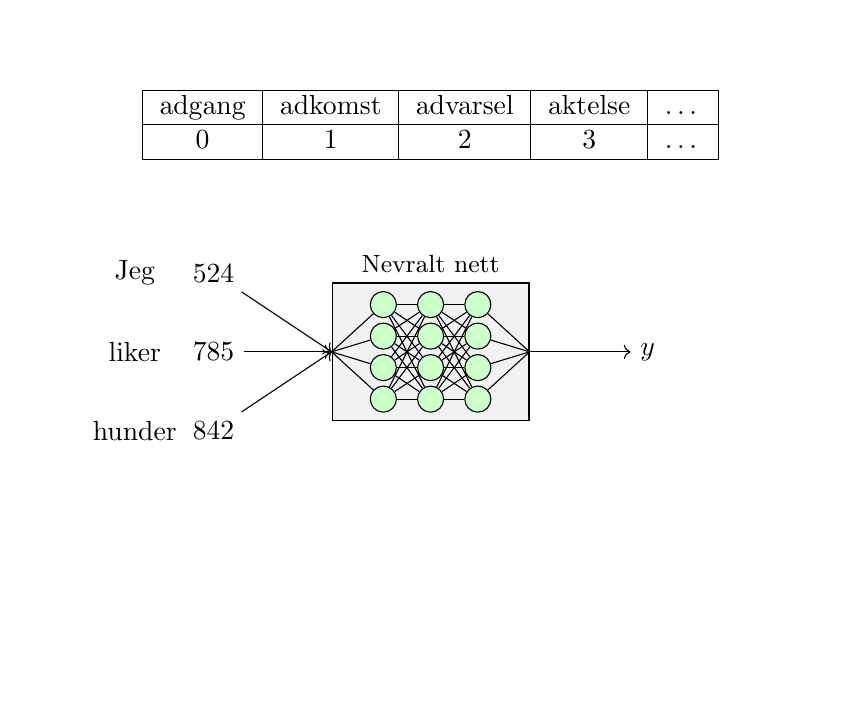
\begin{tikzpicture}
			\node[
				draw=black,
				minimum width=2.5cm,
				minimum height=1.75cm,
				fill=gray!10,
				label=\small{Nevralt nett}
			] (model) at (0, 0) {};
			\node[] (dict) at ($ (model.north) + (0, 2) $) {
				\begin{tabular}{|c|c|c|c|c|}
					\hline
					adgang&adkomst&advarsel&aktelse&\ldots\\
					\hline
					0&1&2&3&\ldots\\
					\hline
				\end{tabular}
			};
			\node[] (x0) at ($ (model.west) - (1.5, -1) $) {$524$};
			\node[] (x1) at ($ (model.west) - (1.5, 0) $) {$785$};
			\node[] (x2) at ($ (model.west) - (1.5, 1) $) {$842$};
			\node[] (w0) at ($ (model.west) - (2.5, -1) $) {Jeg};
			\node[] (w1) at ($ (model.west) - (2.5, 0) $) {liker};
			\node[] (w2) at ($ (model.west) - (2.5, 1) $) {hunder};
			\node[] (output) at ($ (model.east) + (1.5, 0) $) {$y$};
			\draw[->] (x0) -- (model.west);
			\draw[->] (x1) -- (model.west);
			\draw[->] (x2) -- (model.west);
			\draw[->] (model) -- (output);
			\node[] at (-5, -4) {};
			\node[] at (5, 4) {};
			\node[circle, draw=black, fill=green!20] (n11) at ($ (model) + (0, 0.2) $) {};
			\node[circle, draw=black, fill=green!20] (n12) at ($ (model) + (0, -0.2) $) {};
			\node[circle, draw=black, fill=green!20] (n10) at ($ (model) + (0, 0.6) $) {};
			\node[circle, draw=black, fill=green!20] (n13) at ($ (model) + (0, -0.6) $) {};

			\node[circle, draw=black, fill=green!20] (n01) at ($ (model) + (-0.6, 0.2) $) {};
			\node[circle, draw=black, fill=green!20] (n02) at ($ (model) + (-0.6, -0.2) $) {};
			\node[circle, draw=black, fill=green!20] (n00) at ($ (model) + (-0.6, 0.6) $) {};
			\node[circle, draw=black, fill=green!20] (n03) at ($ (model) + (-0.6, -0.6) $) {};


			\node[circle, draw=black, fill=green!20] (n21) at ($ (model) + (0.6, 0.2) $) {};
			\node[circle, draw=black, fill=green!20] (n22) at ($ (model) + (0.6, -0.2) $) {};
			\node[circle, draw=black, fill=green!20] (n20) at ($ (model) + (0.6, 0.6) $) {};
			\node[circle, draw=black, fill=green!20] (n23) at ($ (model) + (0.6, -0.6) $) {};

			\draw[] (model.west) -- (n00);
			\draw[] (model.west) -- (n01);
			\draw[] (model.west) -- (n02);
			\draw[] (model.west) -- (n03);

			\draw[] (n00) -- (n10);
			\draw[] (n00) -- (n11);
			\draw[] (n00) -- (n12);
			\draw[] (n00) -- (n13);
			\draw[] (n01) -- (n10);
			\draw[] (n01) -- (n11);
			\draw[] (n01) -- (n12);
			\draw[] (n01) -- (n13);
			\draw[] (n02) -- (n10);
			\draw[] (n02) -- (n11);
			\draw[] (n02) -- (n12);
			\draw[] (n02) -- (n13);
			\draw[] (n03) -- (n10);
			\draw[] (n03) -- (n11);
			\draw[] (n03) -- (n12);
			\draw[] (n03) -- (n13);

			\draw[] (n10) -- (n20);
			\draw[] (n10) -- (n21);
			\draw[] (n10) -- (n22);
			\draw[] (n10) -- (n23);
			\draw[] (n11) -- (n20);
			\draw[] (n11) -- (n21);
			\draw[] (n11) -- (n22);
			\draw[] (n11) -- (n23);
			\draw[] (n12) -- (n20);
			\draw[] (n12) -- (n21);
			\draw[] (n12) -- (n22);
			\draw[] (n12) -- (n23);
			\draw[] (n13) -- (n20);
			\draw[] (n13) -- (n21);
			\draw[] (n13) -- (n22);
			\draw[] (n13) -- (n23);

			\draw[] (n20) -- (model.east);
			\draw[] (n21) -- (model.east);
			\draw[] (n22) -- (model.east);
			\draw[] (n23) -- (model.east);

		\end{tikzpicture}
		\vfill
	\end{frame}

	\begin{frame}{Teori: Multitask} % Multivariate regression
		\vfill
		\centering
		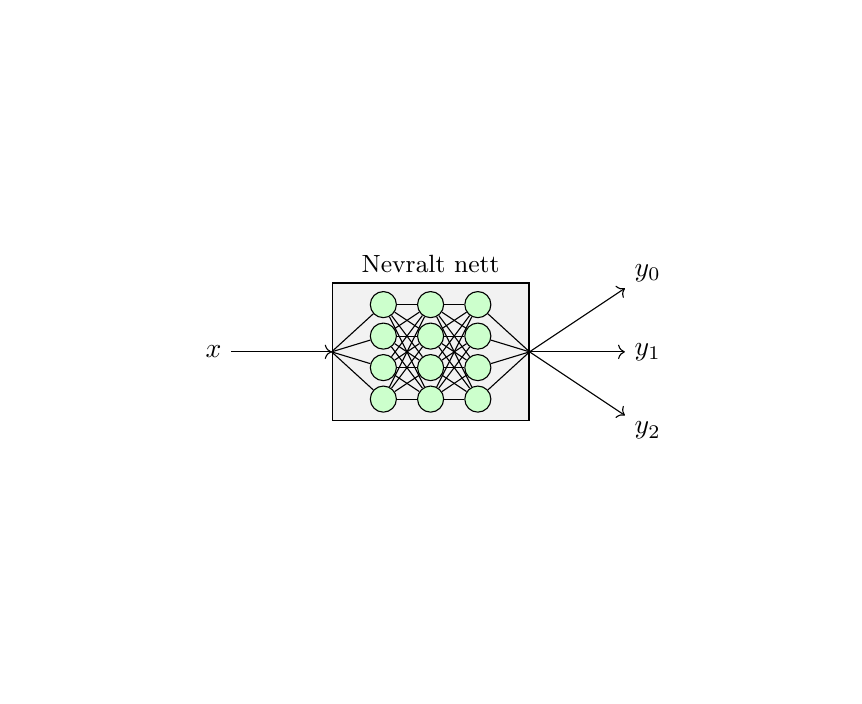
\begin{tikzpicture}
			\node[
				draw=black,
				minimum width=2.5cm,
				minimum height=1.75cm,
				fill=gray!10,
				label=\small{Nevralt nett}
			] (model) at (0, 0) {};
			\node[] (input) at ($ (model.west) - (1.5, 0) $) {$x$};
			\node[] (y0) at ($ (model.east) + (1.5, 1) $) {$y_0$};
			\node[] (y1) at ($ (model.east) + (1.5, 0) $) {$y_1$};
			\node[] (y2) at ($ (model.east) + (1.5, -1) $) {$y_2$};
			\draw[->] (input) -- (model);
			\draw[->] (model.east) -- (y0);
			\draw[->] (model.east) -- (y1);
			\draw[->] (model.east) -- (y2);
			\node[] at (-5, -4) {};
			\node[] at (5, 4) {};
			\node[circle, draw=black, fill=green!20] (n11) at ($ (model) + (0, 0.2) $) {};
			\node[circle, draw=black, fill=green!20] (n12) at ($ (model) + (0, -0.2) $) {};
			\node[circle, draw=black, fill=green!20] (n10) at ($ (model) + (0, 0.6) $) {};
			\node[circle, draw=black, fill=green!20] (n13) at ($ (model) + (0, -0.6) $) {};

			\node[circle, draw=black, fill=green!20] (n01) at ($ (model) + (-0.6, 0.2) $) {};
			\node[circle, draw=black, fill=green!20] (n02) at ($ (model) + (-0.6, -0.2) $) {};
			\node[circle, draw=black, fill=green!20] (n00) at ($ (model) + (-0.6, 0.6) $) {};
			\node[circle, draw=black, fill=green!20] (n03) at ($ (model) + (-0.6, -0.6) $) {};


			\node[circle, draw=black, fill=green!20] (n21) at ($ (model) + (0.6, 0.2) $) {};
			\node[circle, draw=black, fill=green!20] (n22) at ($ (model) + (0.6, -0.2) $) {};
			\node[circle, draw=black, fill=green!20] (n20) at ($ (model) + (0.6, 0.6) $) {};
			\node[circle, draw=black, fill=green!20] (n23) at ($ (model) + (0.6, -0.6) $) {};

			\draw[] (model.west) -- (n00);
			\draw[] (model.west) -- (n01);
			\draw[] (model.west) -- (n02);
			\draw[] (model.west) -- (n03);

			\draw[] (n00) -- (n10);
			\draw[] (n00) -- (n11);
			\draw[] (n00) -- (n12);
			\draw[] (n00) -- (n13);
			\draw[] (n01) -- (n10);
			\draw[] (n01) -- (n11);
			\draw[] (n01) -- (n12);
			\draw[] (n01) -- (n13);
			\draw[] (n02) -- (n10);
			\draw[] (n02) -- (n11);
			\draw[] (n02) -- (n12);
			\draw[] (n02) -- (n13);
			\draw[] (n03) -- (n10);
			\draw[] (n03) -- (n11);
			\draw[] (n03) -- (n12);
			\draw[] (n03) -- (n13);

			\draw[] (n10) -- (n20);
			\draw[] (n10) -- (n21);
			\draw[] (n10) -- (n22);
			\draw[] (n10) -- (n23);
			\draw[] (n11) -- (n20);
			\draw[] (n11) -- (n21);
			\draw[] (n11) -- (n22);
			\draw[] (n11) -- (n23);
			\draw[] (n12) -- (n20);
			\draw[] (n12) -- (n21);
			\draw[] (n12) -- (n22);
			\draw[] (n12) -- (n23);
			\draw[] (n13) -- (n20);
			\draw[] (n13) -- (n21);
			\draw[] (n13) -- (n22);
			\draw[] (n13) -- (n23);

			\draw[] (n20) -- (model.east);
			\draw[] (n21) -- (model.east);
			\draw[] (n22) -- (model.east);
			\draw[] (n23) -- (model.east);

		\end{tikzpicture}
		\vfill
	\end{frame}

	\begin{frame}{Teori: Klassifikasjon} % Classification
		\vfill
		\centering
		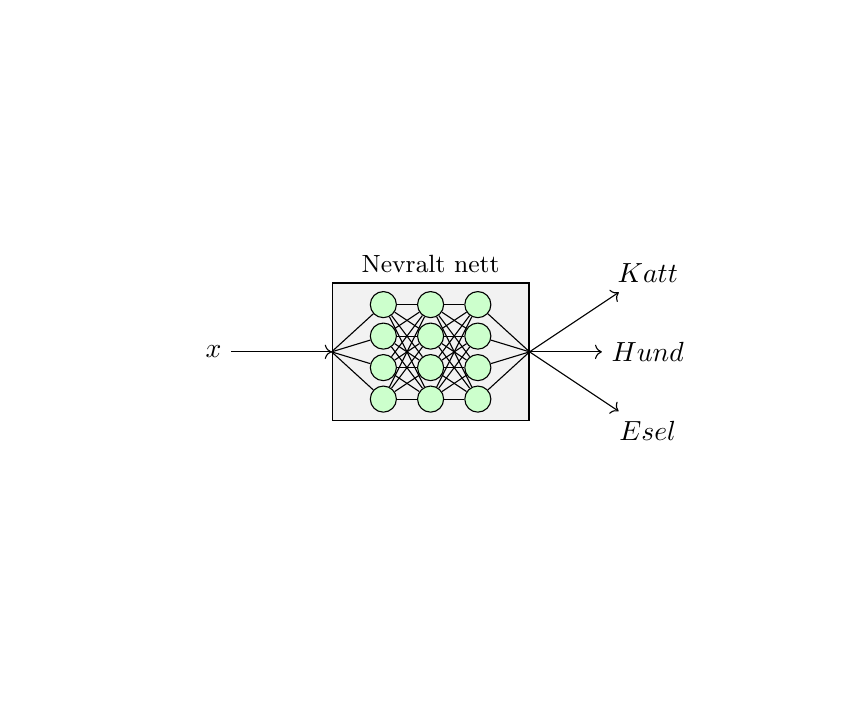
\begin{tikzpicture}
			\node[
				draw=black,
				minimum width=2.5cm,
				minimum height=1.75cm,
				fill=gray!10,
				label=\small{Nevralt nett}
			] (model) at (0, 0) {};
			\node[] (input) at ($ (model.west) - (1.5, 0) $) {$x$};
			\node[] (y0) at ($ (model.east) + (1.5, 1) $) {$Katt$};
			\node[] (y1) at ($ (model.east) + (1.5, 0) $) {$Hund$};
			\node[] (y2) at ($ (model.east) + (1.5, -1) $) {$Esel$};
			\draw[->] (input) -- (model);
			\draw[->] (model.east) -- (y0);
			\draw[->] (model.east) -- (y1);
			\draw[->] (model.east) -- (y2);
			\node[] at (-5, -4) {};
			\node[] at (5, 4) {};
			\node[circle, draw=black, fill=green!20] (n11) at ($ (model) + (0, 0.2) $) {};
			\node[circle, draw=black, fill=green!20] (n12) at ($ (model) + (0, -0.2) $) {};
			\node[circle, draw=black, fill=green!20] (n10) at ($ (model) + (0, 0.6) $) {};
			\node[circle, draw=black, fill=green!20] (n13) at ($ (model) + (0, -0.6) $) {};

			\node[circle, draw=black, fill=green!20] (n01) at ($ (model) + (-0.6, 0.2) $) {};
			\node[circle, draw=black, fill=green!20] (n02) at ($ (model) + (-0.6, -0.2) $) {};
			\node[circle, draw=black, fill=green!20] (n00) at ($ (model) + (-0.6, 0.6) $) {};
			\node[circle, draw=black, fill=green!20] (n03) at ($ (model) + (-0.6, -0.6) $) {};


			\node[circle, draw=black, fill=green!20] (n21) at ($ (model) + (0.6, 0.2) $) {};
			\node[circle, draw=black, fill=green!20] (n22) at ($ (model) + (0.6, -0.2) $) {};
			\node[circle, draw=black, fill=green!20] (n20) at ($ (model) + (0.6, 0.6) $) {};
			\node[circle, draw=black, fill=green!20] (n23) at ($ (model) + (0.6, -0.6) $) {};

			\draw[] (model.west) -- (n00);
			\draw[] (model.west) -- (n01);
			\draw[] (model.west) -- (n02);
			\draw[] (model.west) -- (n03);

			\draw[] (n00) -- (n10);
			\draw[] (n00) -- (n11);
			\draw[] (n00) -- (n12);
			\draw[] (n00) -- (n13);
			\draw[] (n01) -- (n10);
			\draw[] (n01) -- (n11);
			\draw[] (n01) -- (n12);
			\draw[] (n01) -- (n13);
			\draw[] (n02) -- (n10);
			\draw[] (n02) -- (n11);
			\draw[] (n02) -- (n12);
			\draw[] (n02) -- (n13);
			\draw[] (n03) -- (n10);
			\draw[] (n03) -- (n11);
			\draw[] (n03) -- (n12);
			\draw[] (n03) -- (n13);

			\draw[] (n10) -- (n20);
			\draw[] (n10) -- (n21);
			\draw[] (n10) -- (n22);
			\draw[] (n10) -- (n23);
			\draw[] (n11) -- (n20);
			\draw[] (n11) -- (n21);
			\draw[] (n11) -- (n22);
			\draw[] (n11) -- (n23);
			\draw[] (n12) -- (n20);
			\draw[] (n12) -- (n21);
			\draw[] (n12) -- (n22);
			\draw[] (n12) -- (n23);
			\draw[] (n13) -- (n20);
			\draw[] (n13) -- (n21);
			\draw[] (n13) -- (n22);
			\draw[] (n13) -- (n23);

			\draw[] (n20) -- (model.east);
			\draw[] (n21) -- (model.east);
			\draw[] (n22) -- (model.east);
			\draw[] (n23) -- (model.east);

		\end{tikzpicture}
		\vfill
	\end{frame}

	\begin{frame}{Teori: Segmentering} % Segmentation
		\vfill
		\centering
		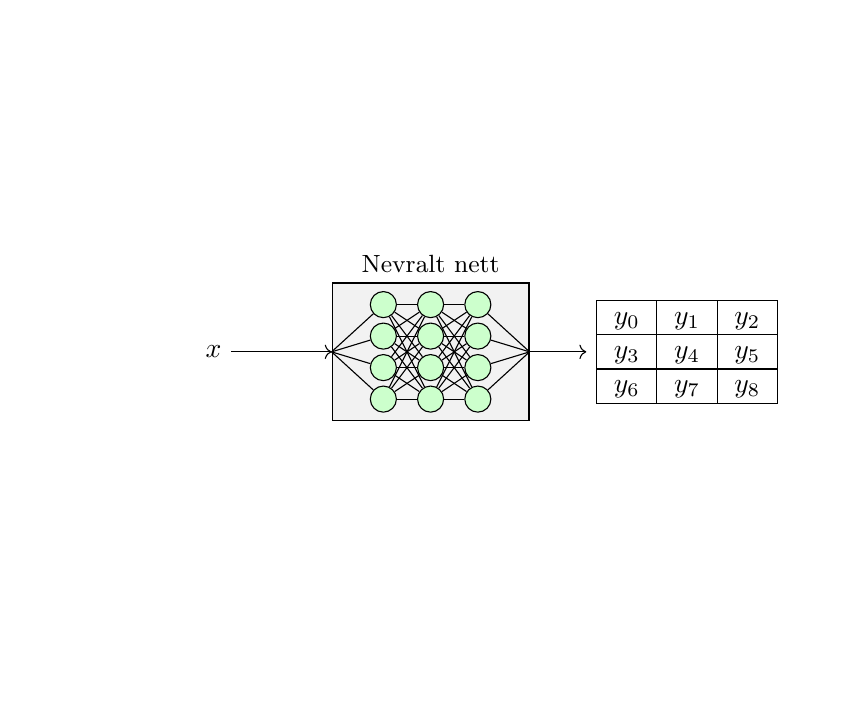
\begin{tikzpicture}
			\node[
				draw=black,
				minimum width=2.5cm,
				minimum height=1.75cm,
				fill=gray!10,
				label=\small{Nevralt nett}
			] (model) at (0, 0) {};
			\node[] (input) at ($ (model.west) - (1.5, 0) $) {$x$};
			\node[] (y) at ($ (model.east) + (2, 0) $) {
				\begin{tabular}{|c|c|c|}
					\hline
					$y_0$&$y_1$&$y_2$\\
					\hline
					$y_3$&$y_4$&$y_5$\\
					\hline
					$y_6$&$y_7$&$y_8$\\
					\hline
				\end{tabular}
			};
			\draw[->] (input) -- (model);
			\draw[->] (model.east) -- (y);
			\node[] at (-5, -4) {};
			\node[] at (5, 4) {};
			\node[circle, draw=black, fill=green!20] (n11) at ($ (model) + (0, 0.2) $) {};
			\node[circle, draw=black, fill=green!20] (n12) at ($ (model) + (0, -0.2) $) {};
			\node[circle, draw=black, fill=green!20] (n10) at ($ (model) + (0, 0.6) $) {};
			\node[circle, draw=black, fill=green!20] (n13) at ($ (model) + (0, -0.6) $) {};

			\node[circle, draw=black, fill=green!20] (n01) at ($ (model) + (-0.6, 0.2) $) {};
			\node[circle, draw=black, fill=green!20] (n02) at ($ (model) + (-0.6, -0.2) $) {};
			\node[circle, draw=black, fill=green!20] (n00) at ($ (model) + (-0.6, 0.6) $) {};
			\node[circle, draw=black, fill=green!20] (n03) at ($ (model) + (-0.6, -0.6) $) {};


			\node[circle, draw=black, fill=green!20] (n21) at ($ (model) + (0.6, 0.2) $) {};
			\node[circle, draw=black, fill=green!20] (n22) at ($ (model) + (0.6, -0.2) $) {};
			\node[circle, draw=black, fill=green!20] (n20) at ($ (model) + (0.6, 0.6) $) {};
			\node[circle, draw=black, fill=green!20] (n23) at ($ (model) + (0.6, -0.6) $) {};

			\draw[] (model.west) -- (n00);
			\draw[] (model.west) -- (n01);
			\draw[] (model.west) -- (n02);
			\draw[] (model.west) -- (n03);

			\draw[] (n00) -- (n10);
			\draw[] (n00) -- (n11);
			\draw[] (n00) -- (n12);
			\draw[] (n00) -- (n13);
			\draw[] (n01) -- (n10);
			\draw[] (n01) -- (n11);
			\draw[] (n01) -- (n12);
			\draw[] (n01) -- (n13);
			\draw[] (n02) -- (n10);
			\draw[] (n02) -- (n11);
			\draw[] (n02) -- (n12);
			\draw[] (n02) -- (n13);
			\draw[] (n03) -- (n10);
			\draw[] (n03) -- (n11);
			\draw[] (n03) -- (n12);
			\draw[] (n03) -- (n13);

			\draw[] (n10) -- (n20);
			\draw[] (n10) -- (n21);
			\draw[] (n10) -- (n22);
			\draw[] (n10) -- (n23);
			\draw[] (n11) -- (n20);
			\draw[] (n11) -- (n21);
			\draw[] (n11) -- (n22);
			\draw[] (n11) -- (n23);
			\draw[] (n12) -- (n20);
			\draw[] (n12) -- (n21);
			\draw[] (n12) -- (n22);
			\draw[] (n12) -- (n23);
			\draw[] (n13) -- (n20);
			\draw[] (n13) -- (n21);
			\draw[] (n13) -- (n22);
			\draw[] (n13) -- (n23);

			\draw[] (n20) -- (model.east);
			\draw[] (n21) -- (model.east);
			\draw[] (n22) -- (model.east);
			\draw[] (n23) -- (model.east);

		\end{tikzpicture}
		\vfill
	\end{frame}

	\begin{frame}{Teori: Emergens}
		\vfill
		\centering
		\begin{tikzpicture}
			\node[] (model) at (0, 0) {};

			\node[inner sep=0pt] (image) at ($ (model) - (3.5, 0) $) {
				\includegraphics[width=2cm]{data/cat.png}
			};

			\node[circle, draw=black, fill=green!20, inner sep=4pt] (n11) at ($ (model) + (0, 0.4) $) {};
			\node[circle, draw=black, fill=green!20, inner sep=4pt] (n12) at ($ (model) + (0, -0.4) $) {};
			\node[circle, draw=black, fill=green!20, inner sep=4pt] (n10) at ($ (model) + (0, 1.2) $) {};
			\node[circle, draw=black, fill=green!20, inner sep=4pt] (n13) at ($ (model) + (0, -1.2) $) {};

			\node[circle, draw=black, fill=green!20, inner sep=4pt] (n01) at ($ (model) + (-1, 0.4) $) {};
			\node[circle, draw=black, fill=green!20, inner sep=4pt] (n02) at ($ (model) + (-1, -0.4) $) {};
			\node[circle, draw=black, fill=green!20, inner sep=4pt] (n00) at ($ (model) + (-1, 1.2) $) {};
			\node[circle, draw=black, fill=green!20, inner sep=4pt] (n03) at ($ (model) + (-1, -1.2) $) {};


			\node[circle, draw=black, fill=green!20, inner sep=4pt] (n21) at ($ (model) + (1, 0.4) $) {};
			\node[circle, draw=black, fill=green!20, inner sep=4pt] (n22) at ($ (model) + (1, -0.4) $) {};
			\node[circle, draw=black, fill=green!20, inner sep=4pt] (n20) at ($ (model) + (1, 1.2) $) {};
			\node[circle, draw=black, fill=green!20, inner sep=4pt] (n23) at ($ (model) + (1, -1.2) $) {};

			\node[circle, draw=black, fill=green!20, inner sep=4pt, label=right:Katt] (n30) at ($ (model) + (2, 0.6) $) {};
			\node[circle, draw=black, fill=green!20, inner sep=4pt, label=right:Hund] (n31) at ($ (model) + (2, -0.6) $) {};

			\draw[] (n00) -- (n10);
			\draw[] (n00) -- (n11);
			\draw[] (n00) -- (n12);
			\draw[] (n00) -- (n13);
			\draw[] (n01) -- (n10);
			\draw[] (n01) -- (n11);
			\draw[] (n01) -- (n12);
			\draw[] (n01) -- (n13);
			\draw[] (n02) -- (n10);
			\draw[] (n02) -- (n11);
			\draw[] (n02) -- (n12);
			\draw[] (n02) -- (n13);
			\draw[] (n03) -- (n10);
			\draw[] (n03) -- (n11);
			\draw[] (n03) -- (n12);
			\draw[] (n03) -- (n13);

			\draw[] (n10) -- (n20);
			\draw[] (n10) -- (n21);
			\draw[] (n10) -- (n22);
			\draw[] (n10) -- (n23);
			\draw[] (n11) -- (n20);
			\draw[] (n11) -- (n21);
			\draw[] (n11) -- (n22);
			\draw[] (n11) -- (n23);
			\draw[] (n12) -- (n20);
			\draw[] (n12) -- (n21);
			\draw[] (n12) -- (n22);
			\draw[] (n12) -- (n23);
			\draw[] (n13) -- (n20);
			\draw[] (n13) -- (n21);
			\draw[] (n13) -- (n22);
			\draw[] (n13) -- (n23);

			\draw[] (n20) -- (n30);
			\draw[] (n21) -- (n30);
			\draw[] (n22) -- (n30);
			\draw[] (n23) -- (n30);

			\draw[] (n20) -- (n31);
			\draw[] (n21) -- (n31);
			\draw[] (n22) -- (n31);
			\draw[] (n23) -- (n31);

			\draw[] (image.east) -- (n00);
			\draw[] (image.east) -- (n01);
			\draw[] (image.east) -- (n02);
			\draw[] (image.east) -- (n03);

			\node[] at (-1.5, -2.5) {
				\includegraphics[height=1.2cm]{data/first.png}
			};
			\node[] at (0, -2.5) {
				\includegraphics[height=1.2cm]{data/third.png}
			};
			\node[] at (1.5, -2.5) {
				\includegraphics[height=1.2cm]{data/fifth.png}
			};
		\end{tikzpicture}
		\vfill
	\end{frame}

	\begin{frame}{Data: Egne data}
		\centering
		\begin{tikzpicture}
			\node[] at (0, 0) {
				\includegraphics[width=1cm]{data/patient_0.png}
			};
			\node[] at (0.5, 0.9) {
				\includegraphics[width=1cm]{data/patient_1.png}
			};
			\node[] at (1.3, -0.2) {
				\includegraphics[width=1cm]{data/patient_2.png}
			};
			\node[] at (0.2, -1) {
				\includegraphics[width=1cm]{data/patient_3.png}
			};
			\node[] at (1.4, -1.1) {
				\includegraphics[width=1cm]{data/patient_4.png}
			};
			\node[] at (1.6, 0.65) {
				\includegraphics[width=1cm]{data/control_0.png}
			};
			\node[
				draw=black,
				minimum width=2.8cm,
				text depth=3.2cm
			] (dwh) at (0.8, 0.2) {Datavarehus};

			\node[
				draw=black,
				fill=gray!10,
				rounded corners=0.1cm,
				inner sep=4pt
			] (modelling) at ($ (dwh.east) + (2, 0) $) {Modellering};

			\draw[-Latex, very thick] (dwh) -- (modelling);

		\end{tikzpicture}
	\end{frame}

	\begin{frame}{Data: Åpne data}
		\centering
		\begin{tikzpicture}
			\node[] (p0) at (0, 0) {
				\includegraphics[width=1cm]{data/patient_0.png}
			};
			\node[anchor=south] (p1) at ($ (p0.north east) + (0.02, 0.02) $) {
				\includegraphics[width=1cm]{data/patient_1.png}
			};
			\node[anchor=west] (p2) at ($ (p0.east) + (0.04, 0) $) {
				\includegraphics[width=1cm]{data/patient_2.png}
			};
			\node[
				draw=black,
				minimum width=2.6cm,
				text depth=2cm
			] (ahus) at ($ (p0.north east) + (0.01, 0.14) $) {Ahus};

			\node[] (p3) at ($ (p0.south) + (0, -1.2) $) {
				\includegraphics[width=1cm]{data/patient_3.png}
			};
			\node[anchor=west] (p4) at ($ (p3.east) + (0.02, 0) $) {
				\includegraphics[width=1cm]{data/patient_4.png}
			};
			\node[anchor=north] (c0) at ($ (p3.south) + (0, -0.02) $) {
				\includegraphics[width=1cm]{data/control_0.png}
			};
			\node[anchor=north west] (c1) at ($ (p3.south east) + (0.02, -0.02) $) {
				\includegraphics[width=1cm]{data/control_1.png}
			};
			\node[
				draw=black,
				minimum width=2.6cm,
				text depth=1.9cm,
			] (jh) at ($ (p3.south east) + (0.02, 0.2) $) {
				John Hopkins
			};

			\node[] (c2) at ($ (c0.south) + (0, -1.2) $) {
				\includegraphics[width=1cm]{data/control_2.png}
			};
			\node[anchor=west] (c3) at ($ (c2.east) + (0.02, 0) $) {
				\includegraphics[width=1cm]{data/control_3.png}
			};
			\node[anchor=north] (c4) at ($ (c2.south east) + (0.02, -0.04) $) {
				\includegraphics[width=1cm]{data/patient_4.png}
			};
			\node[
				draw=black,
				minimum width=2.6cm,
				text depth=2cm,
			] (kaggle) at ($ (c2.south east) + (0.02, 0.12) $) {
				kaggle.com
			};

			\node[
				rotate=90,
				anchor=north,
				draw=black,
				fill=blue!10,
				minimum width=3cm
			] (internet) at ($ (jh.east) + (1.5, 0) $) {
				Internett
			};

			\draw[-Latex] (ahus) -- (internet);
			\draw[-Latex] (jh) -- (internet);
			\draw[-Latex] (kaggle) -- (internet);

			\node[
				draw=black,
				fill=gray!10,
				rounded corners=0.1cm,
				inner sep=4pt
			] (modelling) at ($ (internet.south) + (1.5, 0) $) {Modellering};

			\draw[-Latex] (internet) -- (modelling);

		\end{tikzpicture}
	\end{frame}

	\begin{frame}{Data: Transfer learning}
		\centering
		\begin{tikzpicture}
			\node[] (p0) at (0, 0) {
				\includegraphics[width=1cm]{data/patient_0.png}
			};
			\node[anchor=south] (p1) at ($ (p0.north east) + (0.02, 0.02) $) {
				\includegraphics[width=1cm]{data/patient_1.png}
			};
			\node[anchor=west] (p2) at ($ (p0.east) + (0.04, 0) $) {
				\includegraphics[width=1cm]{data/patient_2.png}
			};
			\node[
				draw=black,
				minimum width=2.6cm,
				text depth=2cm
			] (ahus) at ($ (p0.north east) + (0.01, 0.14) $) {Ahus};

			\node[] (p3) at ($ (p0.south) + (0, -1.2) $) {
				\includegraphics[width=1cm]{data/patient_3.png}
			};
			\node[anchor=west] (p4) at ($ (p3.east) + (0.02, 0) $) {
				\includegraphics[width=1cm]{data/patient_4.png}
			};
			\node[anchor=north] (c0) at ($ (p3.south) + (0, -0.02) $) {
				\includegraphics[width=1cm]{data/control_0.png}
			};
			\node[anchor=north west] (c1) at ($ (p3.south east) + (0.02, -0.02) $) {
				\includegraphics[width=1cm]{data/control_1.png}
			};
			\node[
				draw=black,
				minimum width=2.6cm,
				text depth=1.9cm,
			] (jh) at ($ (p3.south east) + (0.02, 0.2) $) {
				John Hopkins
			};

			\node[] (c2) at ($ (c0.south) + (0, -1.2) $) {
				\includegraphics[width=1cm]{data/control_2.png}
			};
			\node[anchor=west] (c3) at ($ (c2.east) + (0.02, 0) $) {
				\includegraphics[width=1cm]{data/control_3.png}
			};
			\node[anchor=north] (c4) at ($ (c2.south east) + (0.02, -0.04) $) {
				\includegraphics[width=1cm]{data/patient_4.png}
			};
			\node[
				draw=black,
				minimum width=2.6cm,
				text depth=2cm,
			] (ous) at ($ (c2.south east) + (0.02, 0.12) $) {
				OUS
			};

			\node[
				rotate=90,
				anchor=north,
				draw=black,
				fill=blue!10,
				minimum width=3cm
			] (internet) at ($ (jh.east) + (1.5, 1.4) $) {
				Internett
			};

			\draw[-Latex] (ahus) -- (internet);
			\draw[-Latex] (jh) -- (internet);

			\node[
				draw=black,
				fill=gray!10,
				rounded corners=0.1cm,
				inner sep=4pt
			] (pretraining) at ($ (internet.south) + (1.5, 0) $) {Pretrening};

			\draw[-Latex] (internet) -- (pretraining);

			\node[
				draw=black,
				fill=gray!10,
				rounded corners=0.1cm,
				inner sep=4pt
			] (finetuning) at ($ (ous.east) + (3.4, 0) $) {Tilpassing};

			\draw[-Latex] (ous) -- (finetuning);
			\draw[-Latex] (pretraining) -- (finetuning);

		\end{tikzpicture}
	\end{frame}

	\begin{frame}{Data: Føderert læring}

		\centering
		\begin{tikzpicture}
			\node[] (p0) at (0, 0) {
				\includegraphics[width=1cm]{data/patient_0.png}
			};
			\node[anchor=south] (p1) at ($ (p0.north east) + (0.02, 0.02) $) {
				\includegraphics[width=1cm]{data/patient_1.png}
			};
			\node[anchor=west] (p2) at ($ (p0.east) + (0.04, 0) $) {
				\includegraphics[width=1cm]{data/patient_2.png}
			};
			\node[
				draw=black,
				minimum width=2.6cm,
				text depth=2cm
			] (ahus) at ($ (p0.north east) + (0.01, 0.14) $) {Ahus};

			\node[] (p3) at ($ (p0.south) + (0, -1.2) $) {
				\includegraphics[width=1cm]{data/patient_3.png}
			};
			\node[anchor=west] (p4) at ($ (p3.east) + (0.02, 0) $) {
				\includegraphics[width=1cm]{data/patient_4.png}
			};
			\node[anchor=north] (c0) at ($ (p3.south) + (0, -0.02) $) {
				\includegraphics[width=1cm]{data/control_0.png}
			};
			\node[anchor=north west] (c1) at ($ (p3.south east) + (0.02, -0.02) $) {
				\includegraphics[width=1cm]{data/control_1.png}
			};
			\node[
				draw=black,
				minimum width=2.6cm,
				text depth=1.9cm,
			] (jh) at ($ (p3.south east) + (0.02, 0.2) $) {
				John Hopkins
			};

			\node[] (c2) at ($ (c0.south) + (0, -1.2) $) {
				\includegraphics[width=1cm]{data/control_2.png}
			};
			\node[anchor=west] (c3) at ($ (c2.east) + (0.02, 0) $) {
				\includegraphics[width=1cm]{data/control_3.png}
			};
			\node[anchor=north] (c4) at ($ (c2.south east) + (0.02, -0.04) $) {
				\includegraphics[width=1cm]{data/patient_4.png}
			};
			\node[
				draw=black,
				minimum width=2.6cm,
				text depth=2cm,
			] (kaggle) at ($ (c2.south east) + (0.02, 0.12) $) {
				OUS
			};

			\node[
				draw=black,
				fill=gray!10,
				rounded corners=0.1cm,
				inner sep=4pt
			] (modelling) at ($ (jh.east) + (2.5, 0) $) {Modellering};

			\draw[Latex-] (ahus) -- (modelling);
			\draw[Latex-] (jh) -- (modelling);
			\draw[Latex-] (kaggle) -- (modelling);

		\end{tikzpicture}
	\end{frame}

	\begin{frame}{Utvikling av KI}
		\centering
		\begin{enumerate}
			\item Samle data
			\item Forbered data for trening
			\item Tren modeller
			\item Sammenlign modeller og velg den beste (validering)
			\item Test hvor bra modellen gjør det (testing)
			\item Implementer modellen inn i et sluttbrukersystem
			\item Sluttbrukertesting
			\item Kontinuerlig monitorering
		\end{enumerate}
	\end{frame}

	\begin{frame}{Forklarbar KI}
		\centering
		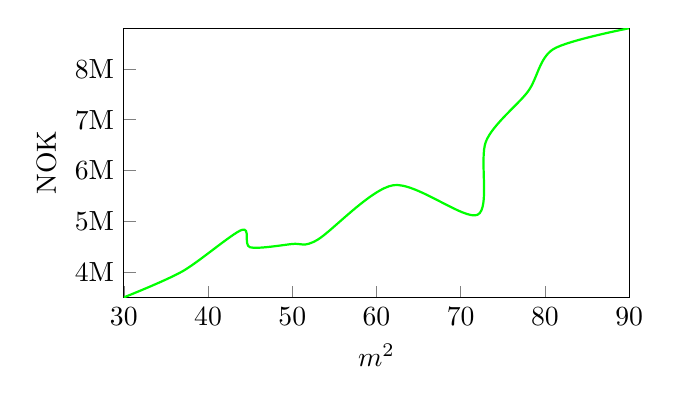
\begin{tikzpicture}
			\begin{axis}[
				xlabel=$m^2$,
				ylabel=NOK,
				ytick={4000000, 5000000, 6000000, 7000000, 8000000},
				yticklabels={4M, 5M, 6M, 7M, 8M},
				scaled y ticks=false,
				xtick pos=bottom,
				ytick pos=left,
				xmin=30,
				xmax=90,,
				ymin=3500000,
				ymax=8800000,
				height=5cm,
				width=8cm
			]
				\addplot[
					smooth,
					green,
					thick
				] coordinates {
					(30, 3500000)
					(37, 4016520)
					(44, 4828170)
					(45, 4486654)
					(50, 4552170)
					(53, 4634912)
					(62, 5709276)
					(72, 5127379)
					(73, 6572351)
					(78, 7557770)
					(81, 8388570)
					(90, 8800000)
				};

				\newcommand{\loss}[2]{
					\addplot[dashed, red] coordinates {
						(####1, 3500000 + ####1 * 30000)
						(####1, ####2)
					};
				}

				\coordinate (center) at (axis cs: 60, 3500000);
			\end{axis}
		\end{tikzpicture}
	\end{frame}

	\begin{frame}{Forklarbar KI}
		\centering
		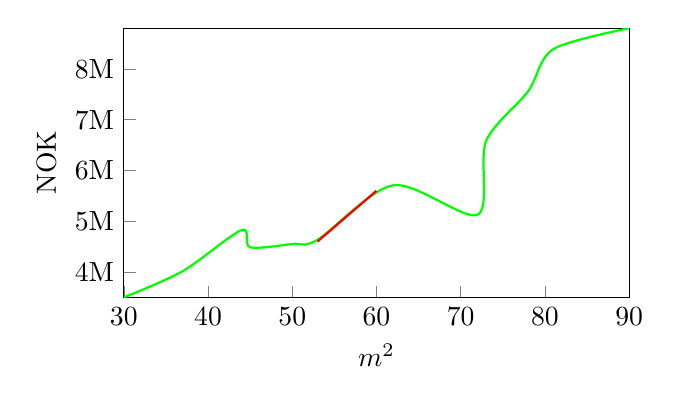
\begin{tikzpicture}
			\begin{axis}[
				xlabel=$m^2$,
				ylabel=NOK,
				ytick={4000000, 5000000, 6000000, 7000000, 8000000},
				yticklabels={4M, 5M, 6M, 7M, 8M},
				scaled y ticks=false,
				xtick pos=bottom,
				ytick pos=left,
				xmin=30,
				xmax=90,,
				ymin=3500000,
				ymax=8800000,
				height=5cm,
				width=8cm
			]
				\addplot[
					smooth,
					green,
					thick
				] coordinates {
					(30, 3500000)
					(37, 4016520)
					(44, 4828170)
					(45, 4486654)
					(50, 4552170)
					(53, 4634912)
					(62, 5709276)
					(72, 5127379)
					(73, 6572351)
					(78, 7557770)
					(81, 8388570)
					(90, 8800000)
				};
				\addplot[
					red,
					thick
				] coordinates {
					(53, 4600000)
					(60, 5600000)
				};

				\newcommand{\loss}[2]{
					\addplot[dashed, red] coordinates {
						(####1, 3500000 + ####1 * 30000)
						(####1, ####2)
					};
				}

				\coordinate (center) at (axis cs: 60, 3500000);
			\end{axis}
		\end{tikzpicture}
	\end{frame}

	\begin{frame}{Forklarbar KI}
		\centering
		\vfill
		\includegraphics[width=6cm]{data/heatmap.jpeg}
		\vfill
	\end{frame}

	\begin{frame}{Forklarbar AI}
		\centering
		\vfill
		\includegraphics[width=6cm]{data/dementia.png}
		\vfill
	\end{frame}

	\begin{frame}{Forklarbar AI}
		\centering
		\vfill
		\includegraphics[width=6cm]{data/rf.png}
		\vfill
	\end{frame}

	\begin{frame}{Chatbotter} % gpt 3.5
		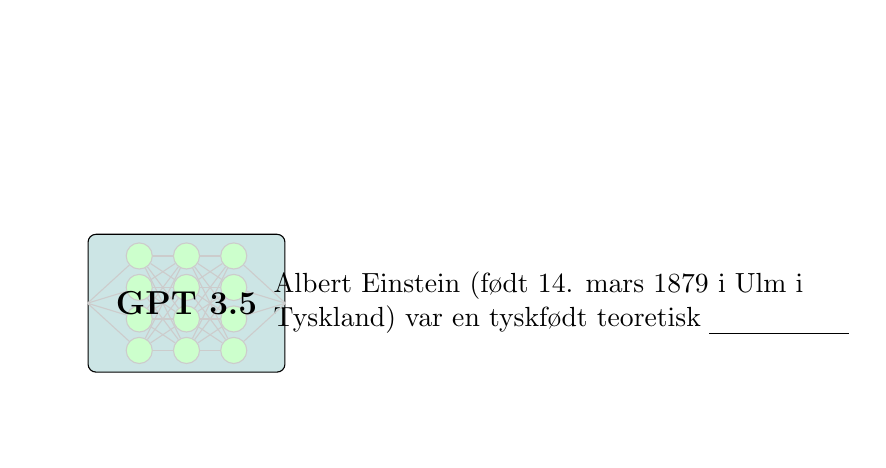
\begin{tikzpicture}
			\node[] at (-1.9, 2.5) {};
			\node[] at (8.3, -2.5) {};
			\node[
				draw=black,
				minimum width=2.5cm,
				minimum height=1.75cm,
				fill=teal!20,
				rounded corners=.1cm,
				anchor=north
			] (model) at (0, 0) {};


			\node[align=left] at ($ (model.east) + (3.5, 0) $) {
				Albert Einstein (født 14. mars 1879 i Ulm i\\ Tyskland) var en tyskfødt teoretisk \uline{\hspace{5em}}
			};

			\node[circle, draw=black!20, fill=green!20] (n11) at ($ (model) + (0, 0.2) $) {};
			\node[circle, draw=black!20, fill=green!20] (n12) at ($ (model) + (0, -0.2) $) {};
			\node[circle, draw=black!20, fill=green!20] (n10) at ($ (model) + (0, 0.6) $) {};
			\node[circle, draw=black!20, fill=green!20] (n13) at ($ (model) + (0, -0.6) $) {};

			\node[circle, draw=black!20, fill=green!20] (n01) at ($ (model) + (-0.6, 0.2) $) {};
			\node[circle, draw=black!20, fill=green!20] (n02) at ($ (model) + (-0.6, -0.2) $) {};
			\node[circle, draw=black!20, fill=green!20] (n00) at ($ (model) + (-0.6, 0.6) $) {};
			\node[circle, draw=black!20, fill=green!20] (n03) at ($ (model) + (-0.6, -0.6) $) {};


			\node[circle, draw=black!20, fill=green!20] (n21) at ($ (model) + (0.6, 0.2) $) {};
			\node[circle, draw=black!20, fill=green!20] (n22) at ($ (model) + (0.6, -0.2) $) {};
			\node[circle, draw=black!20, fill=green!20] (n20) at ($ (model) + (0.6, 0.6) $) {};
			\node[circle, draw=black!20, fill=green!20] (n23) at ($ (model) + (0.6, -0.6) $) {};

			\draw[black!20] (model.west) -- (n00);
			\draw[black!20] (model.west) -- (n01);
			\draw[black!20] (model.west) -- (n02);
			\draw[black!20] (model.west) -- (n03);

			\draw[black!20] (n00) -- (n10);
			\draw[black!20] (n00) -- (n11);
			\draw[black!20] (n00) -- (n12);
			\draw[black!20] (n00) -- (n13);
			\draw[black!20] (n01) -- (n10);
			\draw[black!20] (n01) -- (n11);
			\draw[black!20] (n01) -- (n12);
			\draw[black!20] (n01) -- (n13);
			\draw[black!20] (n02) -- (n10);
			\draw[black!20] (n02) -- (n11);
			\draw[black!20] (n02) -- (n12);
			\draw[black!20] (n02) -- (n13);
			\draw[black!20] (n03) -- (n10);
			\draw[black!20] (n03) -- (n11);
			\draw[black!20] (n03) -- (n12);
			\draw[black!20] (n03) -- (n13);

			\draw[black!20] (n10) -- (n20);
			\draw[black!20] (n10) -- (n21);
			\draw[black!20] (n10) -- (n22);
			\draw[black!20] (n10) -- (n23);
			\draw[black!20] (n11) -- (n20);
			\draw[black!20] (n11) -- (n21);
			\draw[black!20] (n11) -- (n22);
			\draw[black!20] (n11) -- (n23);
			\draw[black!20] (n12) -- (n20);
			\draw[black!20] (n12) -- (n21);
			\draw[black!20] (n12) -- (n22);
			\draw[black!20] (n12) -- (n23);
			\draw[black!20] (n13) -- (n20);
			\draw[black!20] (n13) -- (n21);
			\draw[black!20] (n13) -- (n22);
			\draw[black!20] (n13) -- (n23);

			\draw[black!20] (n20) -- (model.east);
			\draw[black!20] (n21) -- (model.east);
			\draw[black!20] (n22) -- (model.east);
			\draw[black!20] (n23) -- (model.east);

			\node[] at (model) {\large{\textbf{GPT 3.5}}};
		\end{tikzpicture}
	\end{frame}

	\begin{frame}{Chatbotter} % Finetuning
		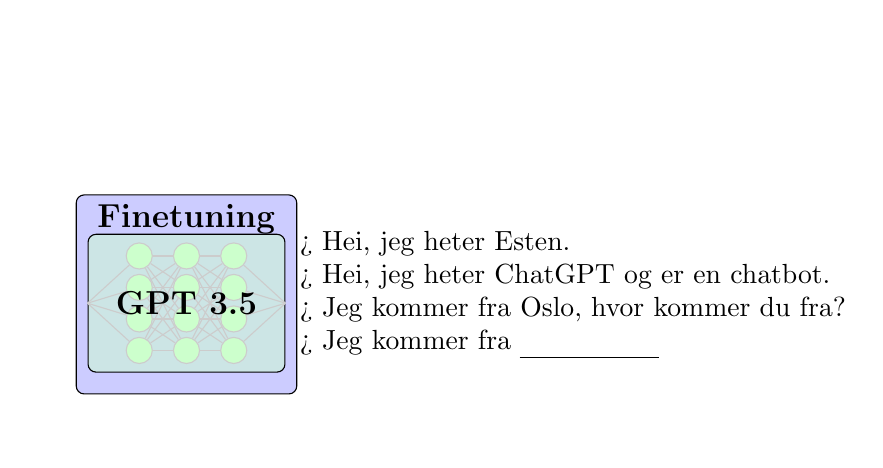
\begin{tikzpicture}
			\node[] at (-1.9, 2.5) {};
			\node[] at (8.3, -2.5) {};
			\node[
				anchor=north,
				draw=black,
				fill=blue!20,
				minimum width=2.8cm,
				text depth=2cm,
				rounded corners=.1cm
			] (finetuning) at (0, 0.5) {\large{\textbf{Finetuning}}};
			\node[
				draw=black,
				minimum width=2.5cm,
				minimum height=1.75cm,
				fill=teal!20,
				rounded corners=.1cm,
				anchor=north
			] (model) at (0, 0) {};


			\node[align=left] at ($ (finetuning.east) + (3.5, 0) $) {
				> Hei, jeg heter Esten.\\
				> Hei, jeg heter ChatGPT og er en chatbot.\\
				> Jeg kommer fra Oslo, hvor kommer du fra?\\
				> Jeg kommer fra \uline{\hspace{5em}}
			};

			\node[circle, draw=black!20, fill=green!20] (n11) at ($ (model) + (0, 0.2) $) {};
			\node[circle, draw=black!20, fill=green!20] (n12) at ($ (model) + (0, -0.2) $) {};
			\node[circle, draw=black!20, fill=green!20] (n10) at ($ (model) + (0, 0.6) $) {};
			\node[circle, draw=black!20, fill=green!20] (n13) at ($ (model) + (0, -0.6) $) {};

			\node[circle, draw=black!20, fill=green!20] (n01) at ($ (model) + (-0.6, 0.2) $) {};
			\node[circle, draw=black!20, fill=green!20] (n02) at ($ (model) + (-0.6, -0.2) $) {};
			\node[circle, draw=black!20, fill=green!20] (n00) at ($ (model) + (-0.6, 0.6) $) {};
			\node[circle, draw=black!20, fill=green!20] (n03) at ($ (model) + (-0.6, -0.6) $) {};


			\node[circle, draw=black!20, fill=green!20] (n21) at ($ (model) + (0.6, 0.2) $) {};
			\node[circle, draw=black!20, fill=green!20] (n22) at ($ (model) + (0.6, -0.2) $) {};
			\node[circle, draw=black!20, fill=green!20] (n20) at ($ (model) + (0.6, 0.6) $) {};
			\node[circle, draw=black!20, fill=green!20] (n23) at ($ (model) + (0.6, -0.6) $) {};

			\draw[black!20] (model.west) -- (n00);
			\draw[black!20] (model.west) -- (n01);
			\draw[black!20] (model.west) -- (n02);
			\draw[black!20] (model.west) -- (n03);

			\draw[black!20] (n00) -- (n10);
			\draw[black!20] (n00) -- (n11);
			\draw[black!20] (n00) -- (n12);
			\draw[black!20] (n00) -- (n13);
			\draw[black!20] (n01) -- (n10);
			\draw[black!20] (n01) -- (n11);
			\draw[black!20] (n01) -- (n12);
			\draw[black!20] (n01) -- (n13);
			\draw[black!20] (n02) -- (n10);
			\draw[black!20] (n02) -- (n11);
			\draw[black!20] (n02) -- (n12);
			\draw[black!20] (n02) -- (n13);
			\draw[black!20] (n03) -- (n10);
			\draw[black!20] (n03) -- (n11);
			\draw[black!20] (n03) -- (n12);
			\draw[black!20] (n03) -- (n13);

			\draw[black!20] (n10) -- (n20);
			\draw[black!20] (n10) -- (n21);
			\draw[black!20] (n10) -- (n22);
			\draw[black!20] (n10) -- (n23);
			\draw[black!20] (n11) -- (n20);
			\draw[black!20] (n11) -- (n21);
			\draw[black!20] (n11) -- (n22);
			\draw[black!20] (n11) -- (n23);
			\draw[black!20] (n12) -- (n20);
			\draw[black!20] (n12) -- (n21);
			\draw[black!20] (n12) -- (n22);
			\draw[black!20] (n12) -- (n23);
			\draw[black!20] (n13) -- (n20);
			\draw[black!20] (n13) -- (n21);
			\draw[black!20] (n13) -- (n22);
			\draw[black!20] (n13) -- (n23);

			\draw[black!20] (n20) -- (model.east);
			\draw[black!20] (n21) -- (model.east);
			\draw[black!20] (n22) -- (model.east);
			\draw[black!20] (n23) -- (model.east);

			\node[] at (model) {\large{\textbf{GPT 3.5}}};
		\end{tikzpicture}
	\end{frame}

	\begin{frame}{Chatbotter} % Reinforcement learning
		\begin{tikzpicture}
			\node[] at (-1.9, 2.5) {};
			\node[] at (8.3, -2.5) {};
			\node[
				anchor=north,
				draw=black,
				fill=purple!20,
				minimum width=3.1cm,
				text depth=2.7cm,
				align=center,
				rounded corners=.1cm
			] (rl) at (0, 1.4) {\large{\textbf{Reinforcement}}\\ \large{\textbf{learning}}};
			\node[
				anchor=north,
				draw=black,
				fill=blue!20,
				minimum width=2.8cm,
				text depth=2cm,
				rounded corners=.1cm
			] (finetuning) at (0, 0.5) {\large{\textbf{Finetuning}}};
			\node[
				draw=black,
				minimum width=2.5cm,
				minimum height=1.75cm,
				fill=teal!20,
				rounded corners=.1cm,
				anchor=north
			] (model) at (0, 0) {};


			\node[align=left] at ($ (rl.east) + (3.5, 0) $) {
				> Hvem er Jonas Gahr St{\o}re?\\
				\textcolor{red}{\faTimesCircle} Jeg interesserer meg ikke s{\aa} mye for politikk.\\
				\textcolor{green}{\faCheckCircle} Jonas Gahr St{\o}re er statsminister i Norge.\\
				\textcolor{red}{\faTimesCircle} Jeg gidder ikke snakke med deg.
			};

			\node[circle, draw=black!20, fill=green!20] (n11) at ($ (model) + (0, 0.2) $) {};
			\node[circle, draw=black!20, fill=green!20] (n12) at ($ (model) + (0, -0.2) $) {};
			\node[circle, draw=black!20, fill=green!20] (n10) at ($ (model) + (0, 0.6) $) {};
			\node[circle, draw=black!20, fill=green!20] (n13) at ($ (model) + (0, -0.6) $) {};

			\node[circle, draw=black!20, fill=green!20] (n01) at ($ (model) + (-0.6, 0.2) $) {};
			\node[circle, draw=black!20, fill=green!20] (n02) at ($ (model) + (-0.6, -0.2) $) {};
			\node[circle, draw=black!20, fill=green!20] (n00) at ($ (model) + (-0.6, 0.6) $) {};
			\node[circle, draw=black!20, fill=green!20] (n03) at ($ (model) + (-0.6, -0.6) $) {};


			\node[circle, draw=black!20, fill=green!20] (n21) at ($ (model) + (0.6, 0.2) $) {};
			\node[circle, draw=black!20, fill=green!20] (n22) at ($ (model) + (0.6, -0.2) $) {};
			\node[circle, draw=black!20, fill=green!20] (n20) at ($ (model) + (0.6, 0.6) $) {};
			\node[circle, draw=black!20, fill=green!20] (n23) at ($ (model) + (0.6, -0.6) $) {};

			\draw[black!20] (model.west) -- (n00);
			\draw[black!20] (model.west) -- (n01);
			\draw[black!20] (model.west) -- (n02);
			\draw[black!20] (model.west) -- (n03);

			\draw[black!20] (n00) -- (n10);
			\draw[black!20] (n00) -- (n11);
			\draw[black!20] (n00) -- (n12);
			\draw[black!20] (n00) -- (n13);
			\draw[black!20] (n01) -- (n10);
			\draw[black!20] (n01) -- (n11);
			\draw[black!20] (n01) -- (n12);
			\draw[black!20] (n01) -- (n13);
			\draw[black!20] (n02) -- (n10);
			\draw[black!20] (n02) -- (n11);
			\draw[black!20] (n02) -- (n12);
			\draw[black!20] (n02) -- (n13);
			\draw[black!20] (n03) -- (n10);
			\draw[black!20] (n03) -- (n11);
			\draw[black!20] (n03) -- (n12);
			\draw[black!20] (n03) -- (n13);

			\draw[black!20] (n10) -- (n20);
			\draw[black!20] (n10) -- (n21);
			\draw[black!20] (n10) -- (n22);
			\draw[black!20] (n10) -- (n23);
			\draw[black!20] (n11) -- (n20);
			\draw[black!20] (n11) -- (n21);
			\draw[black!20] (n11) -- (n22);
			\draw[black!20] (n11) -- (n23);
			\draw[black!20] (n12) -- (n20);
			\draw[black!20] (n12) -- (n21);
			\draw[black!20] (n12) -- (n22);
			\draw[black!20] (n12) -- (n23);
			\draw[black!20] (n13) -- (n20);
			\draw[black!20] (n13) -- (n21);
			\draw[black!20] (n13) -- (n22);
			\draw[black!20] (n13) -- (n23);

			\draw[black!20] (n20) -- (model.east);
			\draw[black!20] (n21) -- (model.east);
			\draw[black!20] (n22) -- (model.east);
			\draw[black!20] (n23) -- (model.east);

			\node[] at (model) {\large{\textbf{GPT 3.5}}};
		\end{tikzpicture}
	\end{frame}

	\begin{frame}{Chatbotter} % Rules
		\begin{tikzpicture}
			\node[] at (-1.9, 2.5) {};
			\node[] at (8.3, -2.5) {};
			\node[
				anchor=north,
				draw=black,
				fill=red!20,
				minimum width=3.4cm,
				text depth=3.75cm,
				rounded corners=.1cm
			] (rules) at (0, 1.9){\large{\textbf{Rule set}}};
			\node[
				anchor=north,
				draw=black,
				fill=purple!20,
				minimum width=3.1cm,
				text depth=2.7cm,
				align=center,
				rounded corners=.1cm
			] (rl) at (0, 1.4) {\large{\textbf{Reinforcement}}\\ \large{\textbf{learning}}};
			\node[
				anchor=north,
				draw=black,
				fill=blue!20,
				minimum width=2.8cm,
				text depth=2cm,
				rounded corners=.1cm
			] (finetuning) at (0, 0.5) {\large{\textbf{Finetuning}}};
			\node[
				draw=black,
				minimum width=2.5cm,
				minimum height=1.75cm,
				fill=teal!20,
				rounded corners=.1cm,
				anchor=north
			] (model) at (0, 0) {};


			\node[draw=black, inner sep=0pt] at ($ (rules.east) + (3.5, 0) $) {
				\includegraphics[width=6cm]{data/rules.png}
			};

			\node[circle, draw=black!20, fill=green!20] (n11) at ($ (model) + (0, 0.2) $) {};
			\node[circle, draw=black!20, fill=green!20] (n12) at ($ (model) + (0, -0.2) $) {};
			\node[circle, draw=black!20, fill=green!20] (n10) at ($ (model) + (0, 0.6) $) {};
			\node[circle, draw=black!20, fill=green!20] (n13) at ($ (model) + (0, -0.6) $) {};

			\node[circle, draw=black!20, fill=green!20] (n01) at ($ (model) + (-0.6, 0.2) $) {};
			\node[circle, draw=black!20, fill=green!20] (n02) at ($ (model) + (-0.6, -0.2) $) {};
			\node[circle, draw=black!20, fill=green!20] (n00) at ($ (model) + (-0.6, 0.6) $) {};
			\node[circle, draw=black!20, fill=green!20] (n03) at ($ (model) + (-0.6, -0.6) $) {};


			\node[circle, draw=black!20, fill=green!20] (n21) at ($ (model) + (0.6, 0.2) $) {};
			\node[circle, draw=black!20, fill=green!20] (n22) at ($ (model) + (0.6, -0.2) $) {};
			\node[circle, draw=black!20, fill=green!20] (n20) at ($ (model) + (0.6, 0.6) $) {};
			\node[circle, draw=black!20, fill=green!20] (n23) at ($ (model) + (0.6, -0.6) $) {};

			\draw[black!20] (model.west) -- (n00);
			\draw[black!20] (model.west) -- (n01);
			\draw[black!20] (model.west) -- (n02);
			\draw[black!20] (model.west) -- (n03);

			\draw[black!20] (n00) -- (n10);
			\draw[black!20] (n00) -- (n11);
			\draw[black!20] (n00) -- (n12);
			\draw[black!20] (n00) -- (n13);
			\draw[black!20] (n01) -- (n10);
			\draw[black!20] (n01) -- (n11);
			\draw[black!20] (n01) -- (n12);
			\draw[black!20] (n01) -- (n13);
			\draw[black!20] (n02) -- (n10);
			\draw[black!20] (n02) -- (n11);
			\draw[black!20] (n02) -- (n12);
			\draw[black!20] (n02) -- (n13);
			\draw[black!20] (n03) -- (n10);
			\draw[black!20] (n03) -- (n11);
			\draw[black!20] (n03) -- (n12);
			\draw[black!20] (n03) -- (n13);

			\draw[black!20] (n10) -- (n20);
			\draw[black!20] (n10) -- (n21);
			\draw[black!20] (n10) -- (n22);
			\draw[black!20] (n10) -- (n23);
			\draw[black!20] (n11) -- (n20);
			\draw[black!20] (n11) -- (n21);
			\draw[black!20] (n11) -- (n22);
			\draw[black!20] (n11) -- (n23);
			\draw[black!20] (n12) -- (n20);
			\draw[black!20] (n12) -- (n21);
			\draw[black!20] (n12) -- (n22);
			\draw[black!20] (n12) -- (n23);
			\draw[black!20] (n13) -- (n20);
			\draw[black!20] (n13) -- (n21);
			\draw[black!20] (n13) -- (n22);
			\draw[black!20] (n13) -- (n23);

			\draw[black!20] (n20) -- (model.east);
			\draw[black!20] (n21) -- (model.east);
			\draw[black!20] (n22) -- (model.east);
			\draw[black!20] (n23) -- (model.east);

			\node[] at (model) {\large{\textbf{GPT 3.5}}};
		\end{tikzpicture}
	\end{frame}

	\begin{frame}{Chatbotter} % Interface
		\begin{tikzpicture}
			\node[] at (-1.9, 2.5) {};
			\node[] at (8.3, -2.5) {};
			\node[
				anchor=north,
				draw=black,
				fill=orange!20,
				minimum width=3.7cm,
				text depth=4.4cm,
				rounded corners=.1cm
			] (interface) at (0, 2.4){\large{\textbf{Interface}}};
			\node[
				anchor=north,
				draw=black,
				fill=red!20,
				minimum width=3.4cm,
				text depth=3.75cm,
				rounded corners=.1cm
			] (rules) at (0, 1.9){\large{\textbf{Rule set}}};
			\node[
				anchor=north,
				draw=black,
				fill=purple!20,
				minimum width=3.1cm,
				text depth=2.7cm,
				align=center,
				rounded corners=.1cm
			] (rl) at (0, 1.4) {\large{\textbf{Reinforcement}}\\ \large{\textbf{learning}}};
			\node[
				anchor=north,
				draw=black,
				fill=blue!20,
				minimum width=2.8cm,
				text depth=2cm,
				rounded corners=.1cm
			] (finetuning) at (0, 0.5) {\large{\textbf{Finetuning}}};
			\node[
				draw=black,
				minimum width=2.5cm,
				minimum height=1.75cm,
				fill=teal!20,
				rounded corners=.1cm,
				anchor=north
			] (model) at (0, 0) {};


			\node[draw=black, inner sep=0pt] at ($ (interface.east) + (3.5, 0) $) {
				\includegraphics[width=6cm]{data/instructions.png}
			};

			\node[circle, draw=black!20, fill=green!20] (n11) at ($ (model) + (0, 0.2) $) {};
			\node[circle, draw=black!20, fill=green!20] (n12) at ($ (model) + (0, -0.2) $) {};
			\node[circle, draw=black!20, fill=green!20] (n10) at ($ (model) + (0, 0.6) $) {};
			\node[circle, draw=black!20, fill=green!20] (n13) at ($ (model) + (0, -0.6) $) {};

			\node[circle, draw=black!20, fill=green!20] (n01) at ($ (model) + (-0.6, 0.2) $) {};
			\node[circle, draw=black!20, fill=green!20] (n02) at ($ (model) + (-0.6, -0.2) $) {};
			\node[circle, draw=black!20, fill=green!20] (n00) at ($ (model) + (-0.6, 0.6) $) {};
			\node[circle, draw=black!20, fill=green!20] (n03) at ($ (model) + (-0.6, -0.6) $) {};


			\node[circle, draw=black!20, fill=green!20] (n21) at ($ (model) + (0.6, 0.2) $) {};
			\node[circle, draw=black!20, fill=green!20] (n22) at ($ (model) + (0.6, -0.2) $) {};
			\node[circle, draw=black!20, fill=green!20] (n20) at ($ (model) + (0.6, 0.6) $) {};
			\node[circle, draw=black!20, fill=green!20] (n23) at ($ (model) + (0.6, -0.6) $) {};

			\draw[black!20] (model.west) -- (n00);
			\draw[black!20] (model.west) -- (n01);
			\draw[black!20] (model.west) -- (n02);
			\draw[black!20] (model.west) -- (n03);

			\draw[black!20] (n00) -- (n10);
			\draw[black!20] (n00) -- (n11);
			\draw[black!20] (n00) -- (n12);
			\draw[black!20] (n00) -- (n13);
			\draw[black!20] (n01) -- (n10);
			\draw[black!20] (n01) -- (n11);
			\draw[black!20] (n01) -- (n12);
			\draw[black!20] (n01) -- (n13);
			\draw[black!20] (n02) -- (n10);
			\draw[black!20] (n02) -- (n11);
			\draw[black!20] (n02) -- (n12);
			\draw[black!20] (n02) -- (n13);
			\draw[black!20] (n03) -- (n10);
			\draw[black!20] (n03) -- (n11);
			\draw[black!20] (n03) -- (n12);
			\draw[black!20] (n03) -- (n13);

			\draw[black!20] (n10) -- (n20);
			\draw[black!20] (n10) -- (n21);
			\draw[black!20] (n10) -- (n22);
			\draw[black!20] (n10) -- (n23);
			\draw[black!20] (n11) -- (n20);
			\draw[black!20] (n11) -- (n21);
			\draw[black!20] (n11) -- (n22);
			\draw[black!20] (n11) -- (n23);
			\draw[black!20] (n12) -- (n20);
			\draw[black!20] (n12) -- (n21);
			\draw[black!20] (n12) -- (n22);
			\draw[black!20] (n12) -- (n23);
			\draw[black!20] (n13) -- (n20);
			\draw[black!20] (n13) -- (n21);
			\draw[black!20] (n13) -- (n22);
			\draw[black!20] (n13) -- (n23);

			\draw[black!20] (n20) -- (model.east);
			\draw[black!20] (n21) -- (model.east);
			\draw[black!20] (n22) -- (model.east);
			\draw[black!20] (n23) -- (model.east);

			\node[] at (model) {\large{\textbf{GPT 3.5}}};
		\end{tikzpicture}
	\end{frame}

	\begin{frame}{Chatbotter} % Bad examples
		\begin{tikzpicture}
			\node[] at (0, -0.8) {
				\includegraphics[width=2.8cm]{data/marriage.png}
			};

			\node[] at (-2.7, -3.7) {
				\includegraphics[width=5cm]{data/angry.jpeg}
			};

			\node[] at (2.7, -3.7) {
				\includegraphics[width=5cm]{data/existential.jpeg}
			};
		\end{tikzpicture}
	\end{frame}

	\begin{frame}{Chatbotter} % Hallucinations
		\centering
		\vfill
		\includegraphics[width=5cm]{data/halluciation.png}
		\vfill
	\end{frame}

	\begin{frame}{Chatbotter} % Parrot
		\centering
		\vfill
		\includegraphics[width=5cm]{data/parrot.png}
		\vfill
	\end{frame}

	\begin{frame}{Fremtiden}
		\centering
		\vfill
		\includegraphics[width=7cm]{data/hockeystick.png}
		\vfill
	\end{frame}
\end{document}
